\documentclass{book}
\usepackage[a4paper,top=2.5cm,bottom=2.5cm,left=2.5cm,right=2.5cm]{geometry}
\usepackage{makeidx}
\usepackage{natbib}
\usepackage{graphicx}
\usepackage{multicol}
\usepackage{float}
\usepackage{listings}
\usepackage{color}
\usepackage{ifthen}
\usepackage[table]{xcolor}
\usepackage{textcomp}
\usepackage{alltt}
\usepackage{ifpdf}
\ifpdf
\usepackage[pdftex,
            pagebackref=true,
            colorlinks=true,
            linkcolor=blue,
            unicode
           ]{hyperref}
\else
\usepackage[ps2pdf,
            pagebackref=true,
            colorlinks=true,
            linkcolor=blue,
            unicode
           ]{hyperref}
\usepackage{pspicture}
\fi
\usepackage[utf8]{inputenc}
\usepackage[french]{babel}

\usepackage{mathptmx}
\usepackage[scaled=.90]{helvet}
\usepackage{courier}
\usepackage{sectsty}
\usepackage{amssymb}
\usepackage[titles]{tocloft}
\usepackage{doxygen}
\lstset{language=C++,inputencoding=utf8,basicstyle=\footnotesize,breaklines=true,breakatwhitespace=true,tabsize=4,numbers=left }
\makeindex
\setcounter{tocdepth}{3}
\renewcommand{\footrulewidth}{0.4pt}
\renewcommand{\familydefault}{\sfdefault}
\hfuzz=15pt
\setlength{\emergencystretch}{15pt}
\hbadness=750
\tolerance=750
\begin{document}
\hypersetup{pageanchor=false,citecolor=blue}
\begin{titlepage}
\vspace*{7cm}
\begin{center}
{\Large Drone\-Wifi \\[1ex]\large 0.\-5 }\\
\vspace*{1cm}
{\large Généré par Doxygen 1.8.3.1}\\
\vspace*{0.5cm}
{\small Lundi Février 18 2013 13:47:06}\\
\end{center}
\end{titlepage}
\clearemptydoublepage
\pagenumbering{roman}
\tableofcontents
\clearemptydoublepage
\pagenumbering{arabic}
\hypersetup{pageanchor=true,citecolor=blue}
\chapter{Index des modules}
\section{Modules}
Liste de tous les modules \-:\begin{DoxyCompactList}
\item \contentsline{section}{Connexion}{\pageref{group___connexion}}{}
\item \contentsline{section}{U\-D\-P}{\pageref{group___u_d_p}}{}
\item \contentsline{section}{I\-O}{\pageref{group___i_o}}{}
\item \contentsline{section}{A\-T\-Commands}{\pageref{group___a_t_commands}}{}
\end{DoxyCompactList}

\chapter{Index des espaces de nommage}
\section{Liste des espaces de nommage}
Liste de tous les espaces de nommage avec une brève description\-:\begin{DoxyCompactList}
\item\contentsline{section}{\hyperlink{namespace_ui}{Ui} }{\pageref{namespace_ui}}{}
\end{DoxyCompactList}

\chapter{Index hiérarchique}
\section{Hiérarchie des classes}
Cette liste d'héritage est classée approximativement par ordre alphabétique \-:\begin{DoxyCompactList}
\item \contentsline{section}{Q\-Main\-Window}{\pageref{class_q_main_window}}{}
\begin{DoxyCompactList}
\item \contentsline{section}{Main\-Window}{\pageref{class_main_window}}{}
\item \contentsline{section}{navdata\-Window}{\pageref{classnavdata_window}}{}
\end{DoxyCompactList}
\item \contentsline{section}{Q\-Thread}{\pageref{class_q_thread}}{}
\begin{DoxyCompactList}
\item \contentsline{section}{A\-R\-Drone}{\pageref{class_a_r_drone}}{}
\end{DoxyCompactList}
\end{DoxyCompactList}

\chapter{Index des structures de données}
\section{Structures de données}
Liste des structures de données avec une brève description \-:\begin{DoxyCompactList}
\item\contentsline{section}{\hyperlink{structardrone}{ardrone} }{\pageref{structardrone}}{}
\item\contentsline{section}{\hyperlink{class_a_r_drone}{A\-R\-Drone} }{\pageref{class_a_r_drone}}{}
\item\contentsline{section}{\hyperlink{structetat__commandes}{etat\-\_\-commandes} }{\pageref{structetat__commandes}}{}
\item\contentsline{section}{\hyperlink{class_main_window}{Main\-Window} }{\pageref{class_main_window}}{}
\item\contentsline{section}{\hyperlink{classnavdata_window}{navdata\-Window} }{\pageref{classnavdata_window}}{}
\item\contentsline{section}{\hyperlink{class_q_main_window}{Q\-Main\-Window} }{\pageref{class_q_main_window}}{}
\item\contentsline{section}{\hyperlink{class_q_thread}{Q\-Thread} }{\pageref{class_q_thread}}{}
\end{DoxyCompactList}

\chapter{Index des fichiers}
\section{Liste des fichiers}
Liste de tous les fichiers avec une brève description \-:\begin{DoxyCompactList}
\item\contentsline{section}{/media/\-D\-E\-V\-E\-L/\-Projet\-I\-U\-T/\-Drone\-Wifi/sources/keyboard\-Command/\hyperlink{ardrone_8cpp}{ardrone.\-cpp} }{\pageref{ardrone_8cpp}}{}
\item\contentsline{section}{/media/\-D\-E\-V\-E\-L/\-Projet\-I\-U\-T/\-Drone\-Wifi/sources/keyboard\-Command/\hyperlink{ardrone_8h}{ardrone.\-h} }{\pageref{ardrone_8h}}{}
\item\contentsline{section}{/media/\-D\-E\-V\-E\-L/\-Projet\-I\-U\-T/\-Drone\-Wifi/sources/keyboard\-Command/\hyperlink{main_8cpp}{main.\-cpp} }{\pageref{main_8cpp}}{}
\item\contentsline{section}{/media/\-D\-E\-V\-E\-L/\-Projet\-I\-U\-T/\-Drone\-Wifi/sources/keyboard\-Command/\hyperlink{mainwindow_8cpp}{mainwindow.\-cpp} }{\pageref{mainwindow_8cpp}}{}
\item\contentsline{section}{/media/\-D\-E\-V\-E\-L/\-Projet\-I\-U\-T/\-Drone\-Wifi/sources/keyboard\-Command/\hyperlink{mainwindow_8h}{mainwindow.\-h} }{\pageref{mainwindow_8h}}{}
\item\contentsline{section}{/media/\-D\-E\-V\-E\-L/\-Projet\-I\-U\-T/\-Drone\-Wifi/sources/keyboard\-Command/\hyperlink{navdatawindow_8cpp}{navdatawindow.\-cpp} }{\pageref{navdatawindow_8cpp}}{}
\item\contentsline{section}{/media/\-D\-E\-V\-E\-L/\-Projet\-I\-U\-T/\-Drone\-Wifi/sources/keyboard\-Command/\hyperlink{navdatawindow_8h}{navdatawindow.\-h} }{\pageref{navdatawindow_8h}}{}
\item\contentsline{section}{/media/\-D\-E\-V\-E\-L/\-Projet\-I\-U\-T/\-Drone\-Wifi/sources/wifi/\hyperlink{connexion_8c}{connexion.\-c} }{\pageref{connexion_8c}}{}
\end{DoxyCompactList}

\chapter{Documentation des modules}
\hypertarget{group___connexion}{\section{Connexion}
\label{group___connexion}\index{Connexion@{Connexion}}
}
\subsection*{Fonctions}
\begin{DoxyCompactItemize}
\item 
int \hyperlink{group___connexion_ga933f44b3a816d407be7ad49f7544342e}{rxsignal\-\_\-cmp} (far \-\_\-wifi\-\_\-wln\-\_\-scan\-\_\-bss $\ast$a, far \-\_\-wifi\-\_\-wln\-\_\-scan\-\_\-bss $\ast$b)
\begin{DoxyCompactList}\small\item\em fonction qui permet le trie les points d'accès Wi\-Fi par puissance du signal \end{DoxyCompactList}\item 
root void \hyperlink{group___connexion_gad60eefc83c0bcc85273af32869e49f5d}{scan\-\_\-assoc\-\_\-callback} (far wifi\-\_\-scan\-\_\-data $\ast$data)
\begin{DoxyCompactList}\small\item\em fonction de callback qui traite les points d'accès donnés \-: recherche le point d'accès du drone et se connecte \end{DoxyCompactList}\item 
void \hyperlink{group___connexion_ga4316deed036a20c32186612b0e2ed7f2}{connexion} (void)
\begin{DoxyCompactList}\small\item\em fonction qui se connecte au drone. Elle se quitte uniquement si la connexion est effective \end{DoxyCompactList}\end{DoxyCompactItemize}


\subsection{Description détaillée}


\subsection{Documentation des fonctions}
\hypertarget{group___connexion_ga4316deed036a20c32186612b0e2ed7f2}{\index{Connexion@{Connexion}!connexion@{connexion}}
\index{connexion@{connexion}!Connexion@{Connexion}}
\subsubsection[{connexion}]{\setlength{\rightskip}{0pt plus 5cm}void connexion (
\begin{DoxyParamCaption}
\item[{void}]{}
\end{DoxyParamCaption}
)}}\label{group___connexion_ga4316deed036a20c32186612b0e2ed7f2}


fonction qui se connecte au drone. Elle se quitte uniquement si la connexion est effective 

\begin{DoxyAuthor}{Auteur}
Thibaut Marty 
\end{DoxyAuthor}


Définition à la ligne 839 du fichier connexion.\-c.



Voici le graphe d'appel pour cette fonction \-:\nopagebreak
\begin{figure}[H]
\begin{center}
\leavevmode
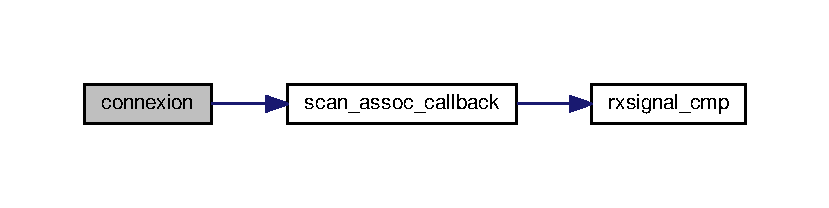
\includegraphics[width=350pt]{group___connexion_ga4316deed036a20c32186612b0e2ed7f2_cgraph}
\end{center}
\end{figure}




Voici le graphe des appelants de cette fonction \-:\nopagebreak
\begin{figure}[H]
\begin{center}
\leavevmode
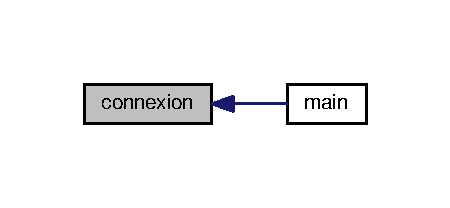
\includegraphics[width=216pt]{group___connexion_ga4316deed036a20c32186612b0e2ed7f2_icgraph}
\end{center}
\end{figure}


\hypertarget{group___connexion_ga933f44b3a816d407be7ad49f7544342e}{\index{Connexion@{Connexion}!rxsignal\-\_\-cmp@{rxsignal\-\_\-cmp}}
\index{rxsignal\-\_\-cmp@{rxsignal\-\_\-cmp}!Connexion@{Connexion}}
\subsubsection[{rxsignal\-\_\-cmp}]{\setlength{\rightskip}{0pt plus 5cm}int rxsignal\-\_\-cmp (
\begin{DoxyParamCaption}
\item[{far \-\_\-wifi\-\_\-wln\-\_\-scan\-\_\-bss $\ast$}]{a, }
\item[{far \-\_\-wifi\-\_\-wln\-\_\-scan\-\_\-bss $\ast$}]{b}
\end{DoxyParamCaption}
)}}\label{group___connexion_ga933f44b3a816d407be7ad49f7544342e}


fonction qui permet le trie les points d'accès Wi\-Fi par puissance du signal 


\begin{DoxyParams}{Paramètres}
{\em a} & un \-\_\-wifi\-\_\-wln\-\_\-scan\-\_\-bss qui correspond à un point d'accès \\
\hline
{\em b} & un \-\_\-wifi\-\_\-wln\-\_\-scan\-\_\-bss qui correspond à un point d'accès \\
\hline
\end{DoxyParams}
\begin{DoxyAuthor}{Auteur}
Dynamic C 
\end{DoxyAuthor}


Définition à la ligne 775 du fichier connexion.\-c.



Voici le graphe des appelants de cette fonction \-:\nopagebreak
\begin{figure}[H]
\begin{center}
\leavevmode
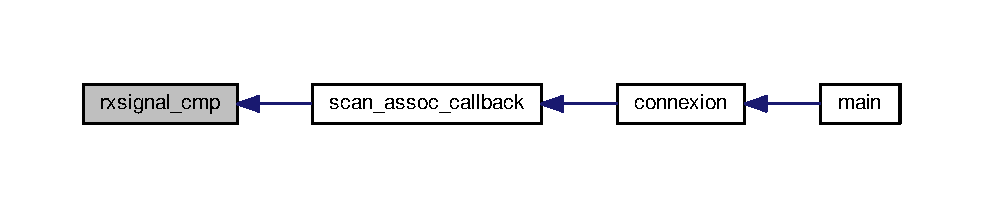
\includegraphics[width=350pt]{group___connexion_ga933f44b3a816d407be7ad49f7544342e_icgraph}
\end{center}
\end{figure}


\hypertarget{group___connexion_gad60eefc83c0bcc85273af32869e49f5d}{\index{Connexion@{Connexion}!scan\-\_\-assoc\-\_\-callback@{scan\-\_\-assoc\-\_\-callback}}
\index{scan\-\_\-assoc\-\_\-callback@{scan\-\_\-assoc\-\_\-callback}!Connexion@{Connexion}}
\subsubsection[{scan\-\_\-assoc\-\_\-callback}]{\setlength{\rightskip}{0pt plus 5cm}root void scan\-\_\-assoc\-\_\-callback (
\begin{DoxyParamCaption}
\item[{far wifi\-\_\-scan\-\_\-data $\ast$}]{data}
\end{DoxyParamCaption}
)}}\label{group___connexion_gad60eefc83c0bcc85273af32869e49f5d}


fonction de callback qui traite les points d'accès donnés \-: recherche le point d'accès du drone et se connecte 


\begin{DoxyParams}{Paramètres}
{\em data} & liste des points d'accès \\
\hline
\end{DoxyParams}
\begin{DoxyAuthor}{Auteur}
Thibaut Marty 
\end{DoxyAuthor}


Définition à la ligne 780 du fichier connexion.\-c.



Voici le graphe d'appel pour cette fonction \-:\nopagebreak
\begin{figure}[H]
\begin{center}
\leavevmode
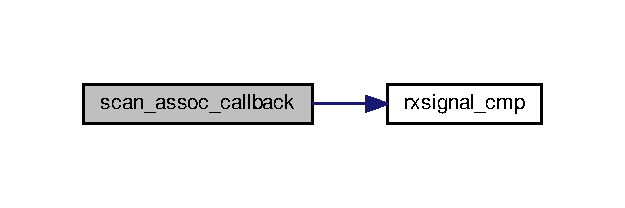
\includegraphics[width=300pt]{group___connexion_gad60eefc83c0bcc85273af32869e49f5d_cgraph}
\end{center}
\end{figure}




Voici le graphe des appelants de cette fonction \-:\nopagebreak
\begin{figure}[H]
\begin{center}
\leavevmode
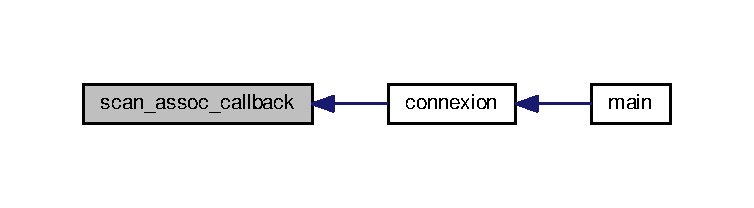
\includegraphics[width=350pt]{group___connexion_gad60eefc83c0bcc85273af32869e49f5d_icgraph}
\end{center}
\end{figure}



\hypertarget{group___u_d_p}{\section{U\-D\-P}
\label{group___u_d_p}\index{U\-D\-P@{U\-D\-P}}
}
\subsection*{Fonctions}
\begin{DoxyCompactItemize}
\item 
\hyperlink{group___a_t_commands_ga58b930fb43c5cd2fc89a84647e6fe51c}{cppbool} \hyperlink{group___u_d_p_ga303d5a717d50385e7908c735d5bddff7}{send\-\_\-packet} (char $\ast$str, const char far $\ast$ip, word port, udp\-\_\-\-Socket $\ast$sock)
\begin{DoxyCompactList}\small\item\em envoie une chaîne de caractère \end{DoxyCompactList}\end{DoxyCompactItemize}


\subsection{Description détaillée}


\subsection{Documentation des fonctions}
\hypertarget{group___u_d_p_ga303d5a717d50385e7908c735d5bddff7}{\index{U\-D\-P@{U\-D\-P}!send\-\_\-packet@{send\-\_\-packet}}
\index{send\-\_\-packet@{send\-\_\-packet}!UDP@{U\-D\-P}}
\subsubsection[{send\-\_\-packet}]{\setlength{\rightskip}{0pt plus 5cm}{\bf cppbool} send\-\_\-packet (
\begin{DoxyParamCaption}
\item[{char $\ast$}]{str, }
\item[{const char far $\ast$}]{ip, }
\item[{word}]{port, }
\item[{udp\-\_\-\-Socket $\ast$}]{sock}
\end{DoxyParamCaption}
)}}\label{group___u_d_p_ga303d5a717d50385e7908c735d5bddff7}


envoie une chaîne de caractère 


\begin{DoxyParams}{Paramètres}
{\em str} & chaîne à envoyé \\
\hline
{\em ip} & ip destination \\
\hline
{\em port} & port de l'envoi \\
\hline
{\em sock} & pointeur sur udp\-\_\-\-Socket utilisée \\
\hline
\end{DoxyParams}
\begin{DoxyReturn}{Renvoie}
true \-: paquet envoyé ; false \-: erreur, la socket est fermée et ne se reouvre pas 
\end{DoxyReturn}
\begin{DoxyAuthor}{Auteur}
Thibaut Marty 
\end{DoxyAuthor}


Définition à la ligne 750 du fichier connexion.\-c.



Voici le graphe des appelants de cette fonction \-:\nopagebreak
\begin{figure}[H]
\begin{center}
\leavevmode
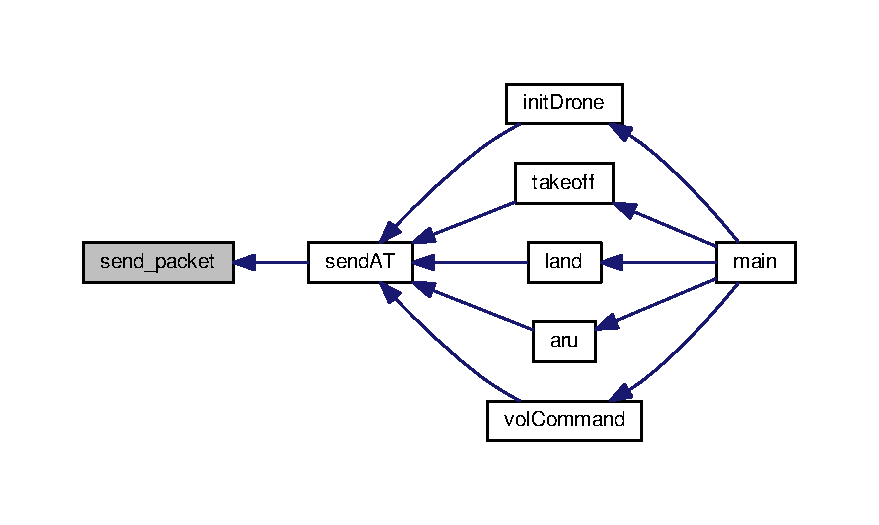
\includegraphics[width=350pt]{group___u_d_p_ga303d5a717d50385e7908c735d5bddff7_icgraph}
\end{center}
\end{figure}



\hypertarget{group___i_o}{\section{I\-O}
\label{group___i_o}\index{I\-O@{I\-O}}
}
\subsection*{Macros}
\begin{DoxyCompactItemize}
\item 
\#define \hyperlink{group___i_o_gad8d73a31b3d7e5ed74e525e198cc78f3}{c\-W\-A\-I\-T\-\_\-5\-\_\-us}
\begin{DoxyCompactList}\small\item\em pause de 5 µs \end{DoxyCompactList}\end{DoxyCompactItemize}
\subsection*{Fonctions}
\begin{DoxyCompactItemize}
\item 
void \hyperlink{group___i_o_ga9cb15ec1781380780672afe306a163ec}{B\-R\-D\-Init} (void)
\begin{DoxyCompactList}\small\item\em Initialise tous les ports d'entreés sorties pour la carte joystick. \end{DoxyCompactList}\item 
void \hyperlink{group___i_o_gaba1669c59c764f752e4759af60633240}{print\-\_\-etat\-\_\-commandes} (\hyperlink{structetat__commandes}{etat\-\_\-commandes} s)
\begin{DoxyCompactList}\small\item\em initialise la structure structure de l'état des commandes \end{DoxyCompactList}\item 
void \hyperlink{group___i_o_ga47503442984c9244a27e7b95ffa472c3}{init\-\_\-etat\-\_\-commandes} (\hyperlink{structetat__commandes}{etat\-\_\-commandes} $\ast$s)
\begin{DoxyCompactList}\small\item\em initialise la structure structure de l'état des commandes \end{DoxyCompactList}\item 
void \hyperlink{group___i_o_gaf61e8f99c1568bc62cd24251e4cc0fa2}{S\-P\-I\-\_\-\-C\-L\-K} (char v)
\begin{DoxyCompactList}\small\item\em modifie l'état de la sortie C\-L\-K pour le convertisseur A/\-N S\-P\-I \end{DoxyCompactList}\item 
void \hyperlink{group___i_o_ga831fe77ab7ce75ba9a41ecb3c08a97d9}{S\-P\-I\-\_\-\-D\-I\-N} (char v)
\begin{DoxyCompactList}\small\item\em modifie l'état de la sortie D\-I\-N pour le convertisseur A/\-N S\-P\-I \end{DoxyCompactList}\item 
void \hyperlink{group___i_o_gab5cfdcd0547c9f87516a805b4849d64f}{S\-P\-I\-\_\-\-C\-S} (char v)
\begin{DoxyCompactList}\small\item\em modifie l'état de la sortie C\-S pour le convertisseur A/\-N S\-P\-I \end{DoxyCompactList}\item 
int \hyperlink{group___i_o_ga837457e63fcbfcc6e59b6d4c59bd7252}{S\-P\-I\-\_\-\-D\-O\-U\-T} (void)
\begin{DoxyCompactList}\small\item\em lit l'état de l'entrée D\-O\-U\-T du convertisseur A/\-N S\-P\-I \end{DoxyCompactList}\item 
void \hyperlink{group___i_o_ga2574e1f1506d0a5313c21891bef79aca}{S\-P\-I\-\_\-delay} (int i)
\begin{DoxyCompactList}\small\item\em temps d'attente de 'i' $\ast$ 5 µs \end{DoxyCompactList}\item 
int \hyperlink{group___i_o_ga5232f075d5cd2577d072721a1494eb03}{S\-P\-Iread} (char addr)
\begin{DoxyCompactList}\small\item\em demande au convertisseur A/\-N S\-P\-I de convertir le canal addr \end{DoxyCompactList}\item 
void \hyperlink{group___i_o_ga91ea6d792c13305827a81e66a1eedf87}{lire\-Commandes} (\hyperlink{structetat__commandes}{etat\-\_\-commandes} $\ast$s)
\begin{DoxyCompactList}\small\item\em remplie la structure de l'état des commandes avec de nouvelles valeurs lues \end{DoxyCompactList}\item 
void \hyperlink{group___i_o_ga85dc4c920777870405563fe56611b457}{ecrire\-Commandes} (\hyperlink{structetat__commandes}{etat\-\_\-commandes} s)
\begin{DoxyCompactList}\small\item\em écris les valeurs de la structure de l'état des commandes en sortie. \end{DoxyCompactList}\end{DoxyCompactItemize}


\subsection{Description détaillée}


\subsection{Documentation des macros}
\hypertarget{group___i_o_gad8d73a31b3d7e5ed74e525e198cc78f3}{\index{I\-O@{I\-O}!c\-W\-A\-I\-T\-\_\-5\-\_\-us@{c\-W\-A\-I\-T\-\_\-5\-\_\-us}}
\index{c\-W\-A\-I\-T\-\_\-5\-\_\-us@{c\-W\-A\-I\-T\-\_\-5\-\_\-us}!IO@{I\-O}}
\subsubsection[{c\-W\-A\-I\-T\-\_\-5\-\_\-us}]{\setlength{\rightskip}{0pt plus 5cm}c\-W\-A\-I\-T\-\_\-5\-\_\-us}}\label{group___i_o_gad8d73a31b3d7e5ed74e525e198cc78f3}
{\bfseries Valeur \-:}
\begin{DoxyCode}
\textcolor{keyword}{asm} ld a,3 $\(\backslash\)
             sub 3 $\(\backslash\)
             ld b,a $\(\backslash\)
             db 0x10,-2
\end{DoxyCode}


pause de 5 µs 

\begin{DoxyAuthor}{Auteur}
Dynamic C 
\end{DoxyAuthor}


Définition à la ligne 151 du fichier connexion.\-c.



\subsection{Documentation des fonctions}
\hypertarget{group___i_o_ga9cb15ec1781380780672afe306a163ec}{\index{I\-O@{I\-O}!B\-R\-D\-Init@{B\-R\-D\-Init}}
\index{B\-R\-D\-Init@{B\-R\-D\-Init}!IO@{I\-O}}
\subsubsection[{B\-R\-D\-Init}]{\setlength{\rightskip}{0pt plus 5cm}void B\-R\-D\-Init (
\begin{DoxyParamCaption}
\item[{void}]{}
\end{DoxyParamCaption}
)}}\label{group___i_o_ga9cb15ec1781380780672afe306a163ec}


Initialise tous les ports d'entreés sorties pour la carte joystick. 

\begin{DoxyAuthor}{Auteur}
Thibaut Marty 
\end{DoxyAuthor}


Définition à la ligne 538 du fichier connexion.\-c.



Voici le graphe des appelants de cette fonction \-:\nopagebreak
\begin{figure}[H]
\begin{center}
\leavevmode
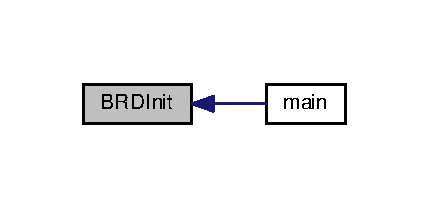
\includegraphics[width=206pt]{group___i_o_ga9cb15ec1781380780672afe306a163ec_icgraph}
\end{center}
\end{figure}


\hypertarget{group___i_o_ga85dc4c920777870405563fe56611b457}{\index{I\-O@{I\-O}!ecrire\-Commandes@{ecrire\-Commandes}}
\index{ecrire\-Commandes@{ecrire\-Commandes}!IO@{I\-O}}
\subsubsection[{ecrire\-Commandes}]{\setlength{\rightskip}{0pt plus 5cm}void ecrire\-Commandes (
\begin{DoxyParamCaption}
\item[{{\bf etat\-\_\-commandes}}]{s}
\end{DoxyParamCaption}
)}}\label{group___i_o_ga85dc4c920777870405563fe56611b457}


écris les valeurs de la structure de l'état des commandes en sortie. 


\begin{DoxyParams}{Paramètres}
{\em \hyperlink{structetat__commandes}{etat\-\_\-commandes}} & structure de l'état des commandes \\
\hline
\end{DoxyParams}
\begin{DoxyAuthor}{Auteur}
Thibaut Marty 
\end{DoxyAuthor}


Définition à la ligne 743 du fichier connexion.\-c.



Voici le graphe des appelants de cette fonction \-:\nopagebreak
\begin{figure}[H]
\begin{center}
\leavevmode
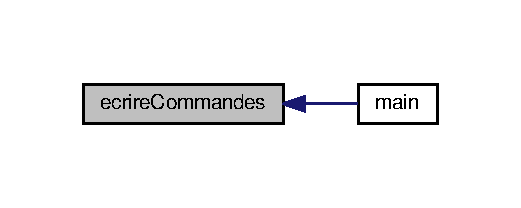
\includegraphics[width=250pt]{group___i_o_ga85dc4c920777870405563fe56611b457_icgraph}
\end{center}
\end{figure}


\hypertarget{group___i_o_ga47503442984c9244a27e7b95ffa472c3}{\index{I\-O@{I\-O}!init\-\_\-etat\-\_\-commandes@{init\-\_\-etat\-\_\-commandes}}
\index{init\-\_\-etat\-\_\-commandes@{init\-\_\-etat\-\_\-commandes}!IO@{I\-O}}
\subsubsection[{init\-\_\-etat\-\_\-commandes}]{\setlength{\rightskip}{0pt plus 5cm}void init\-\_\-etat\-\_\-commandes (
\begin{DoxyParamCaption}
\item[{{\bf etat\-\_\-commandes} $\ast$}]{s}
\end{DoxyParamCaption}
)}}\label{group___i_o_ga47503442984c9244a27e7b95ffa472c3}


initialise la structure structure de l'état des commandes 


\begin{DoxyParams}{Paramètres}
{\em \hyperlink{structetat__commandes}{etat\-\_\-commandes}} & structure de l'état des commandes \\
\hline
\end{DoxyParams}
\begin{DoxyAuthor}{Auteur}
Thibaut Marty 
\end{DoxyAuthor}


Définition à la ligne 604 du fichier connexion.\-c.



Voici le graphe des appelants de cette fonction \-:\nopagebreak
\begin{figure}[H]
\begin{center}
\leavevmode
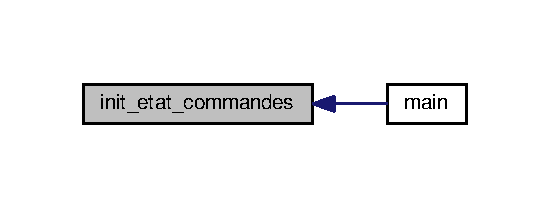
\includegraphics[width=264pt]{group___i_o_ga47503442984c9244a27e7b95ffa472c3_icgraph}
\end{center}
\end{figure}


\hypertarget{group___i_o_ga91ea6d792c13305827a81e66a1eedf87}{\index{I\-O@{I\-O}!lire\-Commandes@{lire\-Commandes}}
\index{lire\-Commandes@{lire\-Commandes}!IO@{I\-O}}
\subsubsection[{lire\-Commandes}]{\setlength{\rightskip}{0pt plus 5cm}void lire\-Commandes (
\begin{DoxyParamCaption}
\item[{{\bf etat\-\_\-commandes} $\ast$}]{s}
\end{DoxyParamCaption}
)}}\label{group___i_o_ga91ea6d792c13305827a81e66a1eedf87}


remplie la structure de l'état des commandes avec de nouvelles valeurs lues 


\begin{DoxyParams}{Paramètres}
{\em \hyperlink{structetat__commandes}{etat\-\_\-commandes}} & structure de l'état des commandes \\
\hline
\end{DoxyParams}
\begin{DoxyAuthor}{Auteur}
Thibaut Marty 
\end{DoxyAuthor}


Définition à la ligne 730 du fichier connexion.\-c.



Voici le graphe d'appel pour cette fonction \-:\nopagebreak
\begin{figure}[H]
\begin{center}
\leavevmode
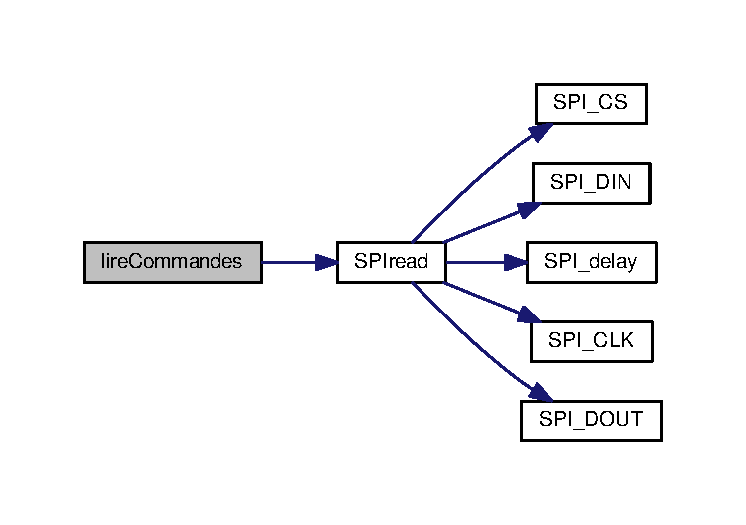
\includegraphics[width=350pt]{group___i_o_ga91ea6d792c13305827a81e66a1eedf87_cgraph}
\end{center}
\end{figure}




Voici le graphe des appelants de cette fonction \-:\nopagebreak
\begin{figure}[H]
\begin{center}
\leavevmode
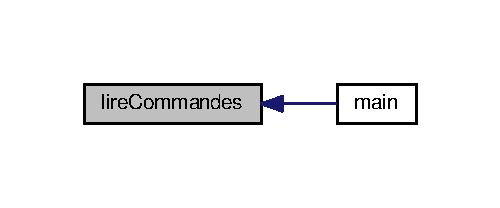
\includegraphics[width=240pt]{group___i_o_ga91ea6d792c13305827a81e66a1eedf87_icgraph}
\end{center}
\end{figure}


\hypertarget{group___i_o_gaba1669c59c764f752e4759af60633240}{\index{I\-O@{I\-O}!print\-\_\-etat\-\_\-commandes@{print\-\_\-etat\-\_\-commandes}}
\index{print\-\_\-etat\-\_\-commandes@{print\-\_\-etat\-\_\-commandes}!IO@{I\-O}}
\subsubsection[{print\-\_\-etat\-\_\-commandes}]{\setlength{\rightskip}{0pt plus 5cm}void print\-\_\-etat\-\_\-commandes (
\begin{DoxyParamCaption}
\item[{{\bf etat\-\_\-commandes}}]{s}
\end{DoxyParamCaption}
)}}\label{group___i_o_gaba1669c59c764f752e4759af60633240}


initialise la structure structure de l'état des commandes 


\begin{DoxyParams}{Paramètres}
{\em \hyperlink{structetat__commandes}{etat\-\_\-commandes}} & structure de l'état des commandes \\
\hline
\end{DoxyParams}
\begin{DoxyAuthor}{Auteur}
Thibaut Marty 
\end{DoxyAuthor}


Définition à la ligne 585 du fichier connexion.\-c.

\hypertarget{group___i_o_gaf61e8f99c1568bc62cd24251e4cc0fa2}{\index{I\-O@{I\-O}!S\-P\-I\-\_\-\-C\-L\-K@{S\-P\-I\-\_\-\-C\-L\-K}}
\index{S\-P\-I\-\_\-\-C\-L\-K@{S\-P\-I\-\_\-\-C\-L\-K}!IO@{I\-O}}
\subsubsection[{S\-P\-I\-\_\-\-C\-L\-K}]{\setlength{\rightskip}{0pt plus 5cm}void S\-P\-I\-\_\-\-C\-L\-K (
\begin{DoxyParamCaption}
\item[{char}]{v}
\end{DoxyParamCaption}
)}}\label{group___i_o_gaf61e8f99c1568bc62cd24251e4cc0fa2}


modifie l'état de la sortie C\-L\-K pour le convertisseur A/\-N S\-P\-I 


\begin{DoxyParams}{Paramètres}
{\em v} & 1 \-: +3.3\-V ; 0 \-: 0\-V \\
\hline
\end{DoxyParams}
\begin{DoxyAuthor}{Auteur}
Thibaut Marty 
\end{DoxyAuthor}


Définition à la ligne 622 du fichier connexion.\-c.



Voici le graphe des appelants de cette fonction \-:\nopagebreak
\begin{figure}[H]
\begin{center}
\leavevmode
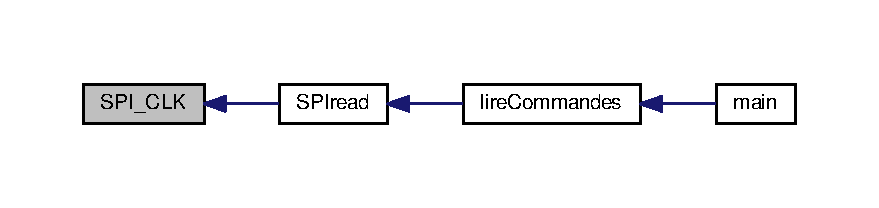
\includegraphics[width=350pt]{group___i_o_gaf61e8f99c1568bc62cd24251e4cc0fa2_icgraph}
\end{center}
\end{figure}


\hypertarget{group___i_o_gab5cfdcd0547c9f87516a805b4849d64f}{\index{I\-O@{I\-O}!S\-P\-I\-\_\-\-C\-S@{S\-P\-I\-\_\-\-C\-S}}
\index{S\-P\-I\-\_\-\-C\-S@{S\-P\-I\-\_\-\-C\-S}!IO@{I\-O}}
\subsubsection[{S\-P\-I\-\_\-\-C\-S}]{\setlength{\rightskip}{0pt plus 5cm}void S\-P\-I\-\_\-\-C\-S (
\begin{DoxyParamCaption}
\item[{char}]{v}
\end{DoxyParamCaption}
)}}\label{group___i_o_gab5cfdcd0547c9f87516a805b4849d64f}


modifie l'état de la sortie C\-S pour le convertisseur A/\-N S\-P\-I 


\begin{DoxyParams}{Paramètres}
{\em v} & 1 \-: +3.3\-V ; 0 \-: 0\-V \\
\hline
\end{DoxyParams}
\begin{DoxyAuthor}{Auteur}
Thibaut Marty 
\end{DoxyAuthor}


Définition à la ligne 623 du fichier connexion.\-c.



Voici le graphe des appelants de cette fonction \-:\nopagebreak
\begin{figure}[H]
\begin{center}
\leavevmode
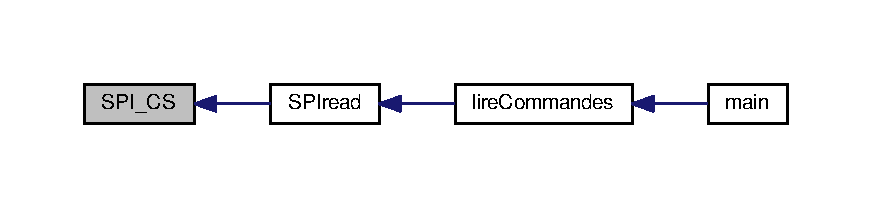
\includegraphics[width=350pt]{group___i_o_gab5cfdcd0547c9f87516a805b4849d64f_icgraph}
\end{center}
\end{figure}


\hypertarget{group___i_o_ga2574e1f1506d0a5313c21891bef79aca}{\index{I\-O@{I\-O}!S\-P\-I\-\_\-delay@{S\-P\-I\-\_\-delay}}
\index{S\-P\-I\-\_\-delay@{S\-P\-I\-\_\-delay}!IO@{I\-O}}
\subsubsection[{S\-P\-I\-\_\-delay}]{\setlength{\rightskip}{0pt plus 5cm}void S\-P\-I\-\_\-delay (
\begin{DoxyParamCaption}
\item[{int}]{i}
\end{DoxyParamCaption}
)}}\label{group___i_o_ga2574e1f1506d0a5313c21891bef79aca}


temps d'attente de 'i' $\ast$ 5 µs 


\begin{DoxyParams}{Paramètres}
{\em i} & \-: nombre d'attente de 5 µs \\
\hline
\end{DoxyParams}
\begin{DoxyAuthor}{Auteur}
Thibaut Marty 
\end{DoxyAuthor}


Définition à la ligne 631 du fichier connexion.\-c.



Voici le graphe des appelants de cette fonction \-:\nopagebreak
\begin{figure}[H]
\begin{center}
\leavevmode
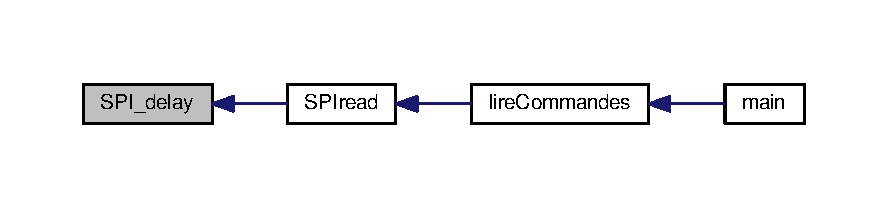
\includegraphics[width=350pt]{group___i_o_ga2574e1f1506d0a5313c21891bef79aca_icgraph}
\end{center}
\end{figure}


\hypertarget{group___i_o_ga831fe77ab7ce75ba9a41ecb3c08a97d9}{\index{I\-O@{I\-O}!S\-P\-I\-\_\-\-D\-I\-N@{S\-P\-I\-\_\-\-D\-I\-N}}
\index{S\-P\-I\-\_\-\-D\-I\-N@{S\-P\-I\-\_\-\-D\-I\-N}!IO@{I\-O}}
\subsubsection[{S\-P\-I\-\_\-\-D\-I\-N}]{\setlength{\rightskip}{0pt plus 5cm}void S\-P\-I\-\_\-\-D\-I\-N (
\begin{DoxyParamCaption}
\item[{char}]{v}
\end{DoxyParamCaption}
)}}\label{group___i_o_ga831fe77ab7ce75ba9a41ecb3c08a97d9}


modifie l'état de la sortie D\-I\-N pour le convertisseur A/\-N S\-P\-I 


\begin{DoxyParams}{Paramètres}
{\em v} & 1 \-: +3.3\-V ; 0 \-: 0\-V \\
\hline
\end{DoxyParams}
\begin{DoxyAuthor}{Auteur}
Thibaut Marty 
\end{DoxyAuthor}


Définition à la ligne 621 du fichier connexion.\-c.



Voici le graphe des appelants de cette fonction \-:\nopagebreak
\begin{figure}[H]
\begin{center}
\leavevmode
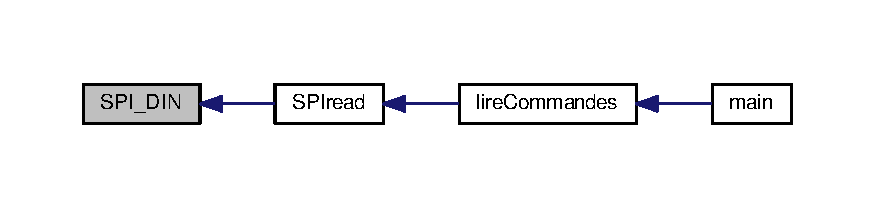
\includegraphics[width=350pt]{group___i_o_ga831fe77ab7ce75ba9a41ecb3c08a97d9_icgraph}
\end{center}
\end{figure}


\hypertarget{group___i_o_ga837457e63fcbfcc6e59b6d4c59bd7252}{\index{I\-O@{I\-O}!S\-P\-I\-\_\-\-D\-O\-U\-T@{S\-P\-I\-\_\-\-D\-O\-U\-T}}
\index{S\-P\-I\-\_\-\-D\-O\-U\-T@{S\-P\-I\-\_\-\-D\-O\-U\-T}!IO@{I\-O}}
\subsubsection[{S\-P\-I\-\_\-\-D\-O\-U\-T}]{\setlength{\rightskip}{0pt plus 5cm}int S\-P\-I\-\_\-\-D\-O\-U\-T (
\begin{DoxyParamCaption}
\item[{void}]{}
\end{DoxyParamCaption}
)}}\label{group___i_o_ga837457e63fcbfcc6e59b6d4c59bd7252}


lit l'état de l'entrée D\-O\-U\-T du convertisseur A/\-N S\-P\-I 

\begin{DoxyReturn}{Renvoie}
1 \-: +3.3\-V ; 0 \-: 0\-V 
\end{DoxyReturn}
\begin{DoxyAuthor}{Auteur}
Thibaut Marty 
\end{DoxyAuthor}


Définition à la ligne 624 du fichier connexion.\-c.



Voici le graphe des appelants de cette fonction \-:\nopagebreak
\begin{figure}[H]
\begin{center}
\leavevmode
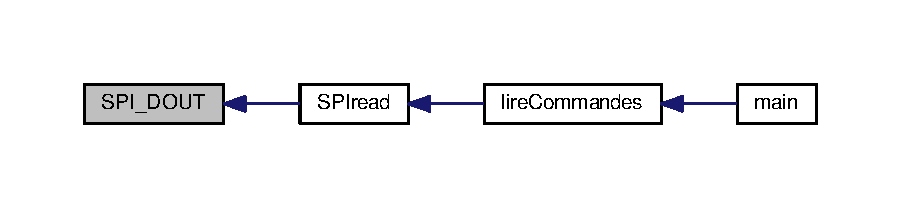
\includegraphics[width=350pt]{group___i_o_ga837457e63fcbfcc6e59b6d4c59bd7252_icgraph}
\end{center}
\end{figure}


\hypertarget{group___i_o_ga5232f075d5cd2577d072721a1494eb03}{\index{I\-O@{I\-O}!S\-P\-Iread@{S\-P\-Iread}}
\index{S\-P\-Iread@{S\-P\-Iread}!IO@{I\-O}}
\subsubsection[{S\-P\-Iread}]{\setlength{\rightskip}{0pt plus 5cm}int S\-P\-Iread (
\begin{DoxyParamCaption}
\item[{char}]{addr}
\end{DoxyParamCaption}
)}}\label{group___i_o_ga5232f075d5cd2577d072721a1494eb03}


demande au convertisseur A/\-N S\-P\-I de convertir le canal addr 


\begin{DoxyParams}{Paramètres}
{\em addr} & canal de lecture (0 à 3) \\
\hline
\end{DoxyParams}
\begin{DoxyReturn}{Renvoie}
le résultat de la conversion 
\end{DoxyReturn}
\begin{DoxyAuthor}{Auteur}
Thibaut Marty 
\end{DoxyAuthor}


Définition à la ligne 638 du fichier connexion.\-c.



Voici le graphe d'appel pour cette fonction \-:\nopagebreak
\begin{figure}[H]
\begin{center}
\leavevmode
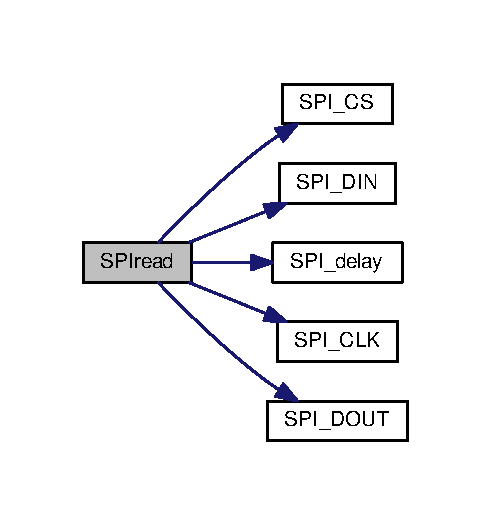
\includegraphics[width=236pt]{group___i_o_ga5232f075d5cd2577d072721a1494eb03_cgraph}
\end{center}
\end{figure}




Voici le graphe des appelants de cette fonction \-:\nopagebreak
\begin{figure}[H]
\begin{center}
\leavevmode
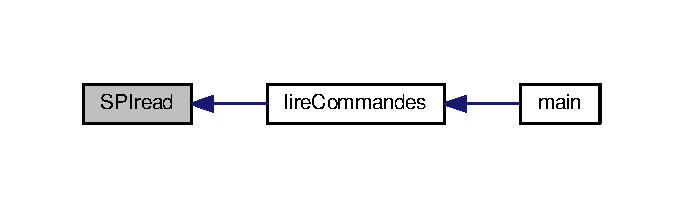
\includegraphics[width=328pt]{group___i_o_ga5232f075d5cd2577d072721a1494eb03_icgraph}
\end{center}
\end{figure}



\hypertarget{group___a_t_commands}{\section{A\-T\-Commands}
\label{group___a_t_commands}\index{A\-T\-Commands@{A\-T\-Commands}}
}
\subsection*{Macros}
\begin{DoxyCompactItemize}
\item 
\#define \hyperlink{group___a_t_commands_ga58b930fb43c5cd2fc89a84647e6fe51c}{cppbool}~char
\begin{DoxyCompactList}\small\item\em Implementation du type c++ bool en c. \end{DoxyCompactList}\end{DoxyCompactItemize}
\subsection*{Fonctions}
\begin{DoxyCompactItemize}
\item 
\hyperlink{group___a_t_commands_ga58b930fb43c5cd2fc89a84647e6fe51c}{cppbool} \hyperlink{group___a_t_commands_gab107cb405a02a0e16ee50f68347c6d4d}{connect\-To\-Drone} (far \hyperlink{structardrone}{ardrone} $\ast$dr)
\begin{DoxyCompactList}\small\item\em Initie la connexion avec le drone dr. \end{DoxyCompactList}\item 
\hyperlink{group___a_t_commands_ga58b930fb43c5cd2fc89a84647e6fe51c}{cppbool} \hyperlink{group___a_t_commands_ga4daa3ada04813c5a99503bd329c6be2c}{init\-Drone} (far \hyperlink{structardrone}{ardrone} $\ast$dr)
\begin{DoxyCompactList}\small\item\em Initialisation du drone dr pour permettre un décollage en toute sécurité. \end{DoxyCompactList}\item 
\hyperlink{group___a_t_commands_ga58b930fb43c5cd2fc89a84647e6fe51c}{cppbool} \hyperlink{group___a_t_commands_ga565736370f76ee54efe74f65acb3ccc4}{takeoff} (far \hyperlink{structardrone}{ardrone} $\ast$dr)
\begin{DoxyCompactList}\small\item\em Commande le décollage du drone dr. \end{DoxyCompactList}\item 
\hyperlink{group___a_t_commands_ga58b930fb43c5cd2fc89a84647e6fe51c}{cppbool} \hyperlink{group___a_t_commands_ga89c4cd20c1bb10d5624cdcc2154efdd1}{land} (far \hyperlink{structardrone}{ardrone} $\ast$dr)
\begin{DoxyCompactList}\small\item\em Commande l'atterissage du drone dr. \end{DoxyCompactList}\item 
\hyperlink{group___a_t_commands_ga58b930fb43c5cd2fc89a84647e6fe51c}{cppbool} \hyperlink{group___a_t_commands_gab16c7bf6e0f5d8df9f422308cb958b2d}{aru} (far \hyperlink{structardrone}{ardrone} $\ast$dr)
\begin{DoxyCompactList}\small\item\em Envoi un arrêt d'urgence au drone dr. \end{DoxyCompactList}\item 
\hyperlink{group___a_t_commands_ga58b930fb43c5cd2fc89a84647e6fe51c}{cppbool} \hyperlink{group___a_t_commands_gafba5305bd996ecb4332a17cf68e79928}{vol\-Command} (far \hyperlink{structardrone}{ardrone} $\ast$dr, float tilt\-Left\-Right\-\_\-, float tilt\-Front\-Back\-\_\-, float go\-Up\-Down\-\_\-, float turn\-Left\-Right\-\_\-)
\begin{DoxyCompactList}\small\item\em Envoi de la commande de vol au drone dr. \end{DoxyCompactList}\item 
void \hyperlink{group___a_t_commands_ga9d9aece95d737ed64ba8e9131ff0065c}{set\-Go\-Up\-Down} (far \hyperlink{structardrone}{ardrone} $\ast$dr, float val)
\begin{DoxyCompactList}\small\item\em Mettre une valeur de manière sécurisée dans le buffer de la vitesse verticale du drone dr. \end{DoxyCompactList}\item 
void \hyperlink{group___a_t_commands_ga0d757863caf7f9c4110ab6e71cac1a4c}{set\-Turn\-Left\-Right} (far \hyperlink{structardrone}{ardrone} $\ast$dr, float val)
\begin{DoxyCompactList}\small\item\em Mettre une valeur dans de manière sécurisée dans le buffer de la vitesse angulaire du drone dr. \end{DoxyCompactList}\item 
void \hyperlink{group___a_t_commands_ga9a290eee046f983fc53d282c0bc53aff}{set\-Tilt\-Front\-Back} (far \hyperlink{structardrone}{ardrone} $\ast$dr, float val)
\begin{DoxyCompactList}\small\item\em Mettre une valeur de manière sécurisé dans le buffer de l'inclinaison avant/arrière du drone dr. \end{DoxyCompactList}\item 
void \hyperlink{group___a_t_commands_ga28a6f7458f7dbcdf7068b26236f10e2c}{set\-Tilt\-Left\-Right} (far \hyperlink{structardrone}{ardrone} $\ast$dr, float val)
\begin{DoxyCompactList}\small\item\em Mettre une valeur de manière sécurisée dans le buffer de l'inclinaison gauche/droite du drone dr. \end{DoxyCompactList}\item 
\hyperlink{group___a_t_commands_ga58b930fb43c5cd2fc89a84647e6fe51c}{cppbool} \hyperlink{group___a_t_commands_gad4a88a78f2b094bcce69b749a845e11c}{send\-A\-T} (far \hyperlink{structardrone}{ardrone} $\ast$dr)
\begin{DoxyCompactList}\small\item\em Envoyer la commande A\-T qui est dans le buffer du drone dr. \end{DoxyCompactList}\item 
far \hyperlink{structardrone}{ardrone} $\ast$ \hyperlink{group___a_t_commands_ga6f1e46bbcb882594c8442c75ae3dedf8}{new\-A\-R\-Drone} (void)
\begin{DoxyCompactList}\small\item\em Constructeur de l'objet ardrone. \end{DoxyCompactList}\item 
void \hyperlink{group___a_t_commands_gad550dbbb88a791f7e8d64c801ce06bf6}{close\-A\-R\-Drone} (far \hyperlink{structardrone}{ardrone} $\ast$dr)
\begin{DoxyCompactList}\small\item\em Destructeur de l'objet ardrone. \end{DoxyCompactList}\end{DoxyCompactItemize}


\subsection{Description détaillée}


\subsection{Documentation des macros}
\hypertarget{group___a_t_commands_ga58b930fb43c5cd2fc89a84647e6fe51c}{\index{A\-T\-Commands@{A\-T\-Commands}!cppbool@{cppbool}}
\index{cppbool@{cppbool}!ATCommands@{A\-T\-Commands}}
\subsubsection[{cppbool}]{\setlength{\rightskip}{0pt plus 5cm}cppbool~char}}\label{group___a_t_commands_ga58b930fb43c5cd2fc89a84647e6fe51c}


Implementation du type c++ bool en c. 

\begin{DoxyAuthor}{Auteur}
Baudouin Feildel 
\end{DoxyAuthor}


Définition à la ligne 83 du fichier connexion.\-c.



\subsection{Documentation des fonctions}
\hypertarget{group___a_t_commands_gab16c7bf6e0f5d8df9f422308cb958b2d}{\index{A\-T\-Commands@{A\-T\-Commands}!aru@{aru}}
\index{aru@{aru}!ATCommands@{A\-T\-Commands}}
\subsubsection[{aru}]{\setlength{\rightskip}{0pt plus 5cm}{\bf cppbool} aru (
\begin{DoxyParamCaption}
\item[{far {\bf ardrone} $\ast$}]{dr}
\end{DoxyParamCaption}
)}}\label{group___a_t_commands_gab16c7bf6e0f5d8df9f422308cb958b2d}


Envoi un arrêt d'urgence au drone dr. 


\begin{DoxyParams}{Paramètres}
{\em far} & ardrone$\ast$ dr \-: Handle du drone \\
\hline
\end{DoxyParams}
\begin{DoxyReturn}{Renvoie}
true \-: arrêt d'urgence envoyé ; false \-: arrêt d'urgence non-\/envoyé 
\end{DoxyReturn}
\begin{DoxyAuthor}{Auteur}
Baudouin Feildel 
\end{DoxyAuthor}


Définition à la ligne 989 du fichier connexion.\-c.



Voici le graphe d'appel pour cette fonction \-:\nopagebreak
\begin{figure}[H]
\begin{center}
\leavevmode
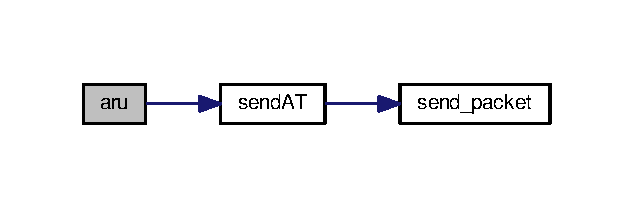
\includegraphics[width=304pt]{group___a_t_commands_gab16c7bf6e0f5d8df9f422308cb958b2d_cgraph}
\end{center}
\end{figure}




Voici le graphe des appelants de cette fonction \-:\nopagebreak
\begin{figure}[H]
\begin{center}
\leavevmode
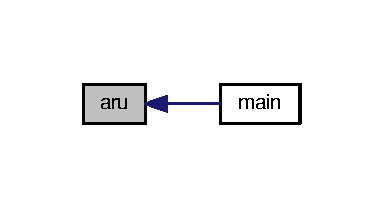
\includegraphics[width=184pt]{group___a_t_commands_gab16c7bf6e0f5d8df9f422308cb958b2d_icgraph}
\end{center}
\end{figure}


\hypertarget{group___a_t_commands_gad550dbbb88a791f7e8d64c801ce06bf6}{\index{A\-T\-Commands@{A\-T\-Commands}!close\-A\-R\-Drone@{close\-A\-R\-Drone}}
\index{close\-A\-R\-Drone@{close\-A\-R\-Drone}!ATCommands@{A\-T\-Commands}}
\subsubsection[{close\-A\-R\-Drone}]{\setlength{\rightskip}{0pt plus 5cm}void close\-A\-R\-Drone (
\begin{DoxyParamCaption}
\item[{far {\bf ardrone} $\ast$}]{dr}
\end{DoxyParamCaption}
)}}\label{group___a_t_commands_gad550dbbb88a791f7e8d64c801ce06bf6}


Destructeur de l'objet ardrone. 


\begin{DoxyParams}{Paramètres}
{\em far} & ardrone$\ast$ dr \-: Handle du objet drone \\
\hline
\end{DoxyParams}
\begin{DoxyAuthor}{Auteur}
Baudouin Feildel 
\end{DoxyAuthor}
\hypertarget{group___a_t_commands_gab107cb405a02a0e16ee50f68347c6d4d}{\index{A\-T\-Commands@{A\-T\-Commands}!connect\-To\-Drone@{connect\-To\-Drone}}
\index{connect\-To\-Drone@{connect\-To\-Drone}!ATCommands@{A\-T\-Commands}}
\subsubsection[{connect\-To\-Drone}]{\setlength{\rightskip}{0pt plus 5cm}{\bf cppbool} connect\-To\-Drone (
\begin{DoxyParamCaption}
\item[{far {\bf ardrone} $\ast$}]{dr}
\end{DoxyParamCaption}
)}}\label{group___a_t_commands_gab107cb405a02a0e16ee50f68347c6d4d}


Initie la connexion avec le drone dr. 


\begin{DoxyParams}{Paramètres}
{\em far} & ardrone$\ast$ dr \-: handle de drone \\
\hline
\end{DoxyParams}
\begin{DoxyReturn}{Renvoie}
true \-: Connexion réussie ; false \-: Connexion échouée 
\end{DoxyReturn}
\begin{DoxyAuthor}{Auteur}
Baudouin Feildel 
\end{DoxyAuthor}


Définition à la ligne 913 du fichier connexion.\-c.



Voici le graphe des appelants de cette fonction \-:\nopagebreak
\begin{figure}[H]
\begin{center}
\leavevmode
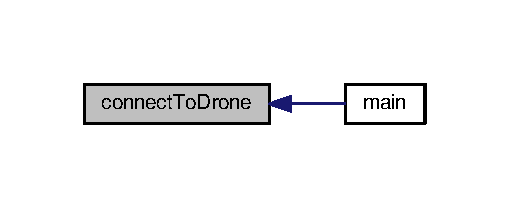
\includegraphics[width=244pt]{group___a_t_commands_gab107cb405a02a0e16ee50f68347c6d4d_icgraph}
\end{center}
\end{figure}


\hypertarget{group___a_t_commands_ga4daa3ada04813c5a99503bd329c6be2c}{\index{A\-T\-Commands@{A\-T\-Commands}!init\-Drone@{init\-Drone}}
\index{init\-Drone@{init\-Drone}!ATCommands@{A\-T\-Commands}}
\subsubsection[{init\-Drone}]{\setlength{\rightskip}{0pt plus 5cm}{\bf cppbool} init\-Drone (
\begin{DoxyParamCaption}
\item[{far {\bf ardrone} $\ast$}]{dr}
\end{DoxyParamCaption}
)}}\label{group___a_t_commands_ga4daa3ada04813c5a99503bd329c6be2c}


Initialisation du drone dr pour permettre un décollage en toute sécurité. 


\begin{DoxyParams}{Paramètres}
{\em far} & ardrone$\ast$ dr \-: Handle du drone \\
\hline
\end{DoxyParams}
\begin{DoxyReturn}{Renvoie}
true \-: initialisation réussie ; false \-: initialisation échouée 
\end{DoxyReturn}
\begin{DoxyAuthor}{Auteur}
Baudouin Feildel 
\end{DoxyAuthor}


Définition à la ligne 935 du fichier connexion.\-c.



Voici le graphe d'appel pour cette fonction \-:\nopagebreak
\begin{figure}[H]
\begin{center}
\leavevmode
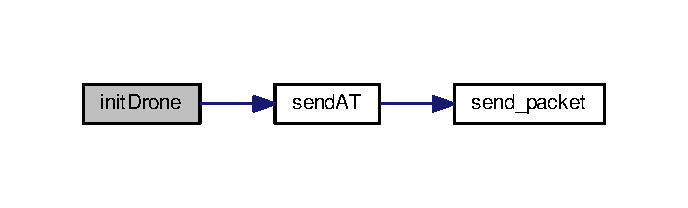
\includegraphics[width=330pt]{group___a_t_commands_ga4daa3ada04813c5a99503bd329c6be2c_cgraph}
\end{center}
\end{figure}




Voici le graphe des appelants de cette fonction \-:\nopagebreak
\begin{figure}[H]
\begin{center}
\leavevmode
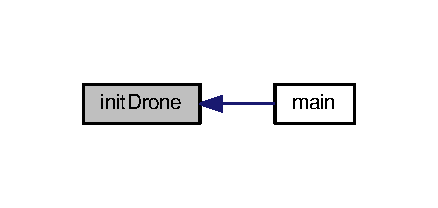
\includegraphics[width=210pt]{group___a_t_commands_ga4daa3ada04813c5a99503bd329c6be2c_icgraph}
\end{center}
\end{figure}


\hypertarget{group___a_t_commands_ga89c4cd20c1bb10d5624cdcc2154efdd1}{\index{A\-T\-Commands@{A\-T\-Commands}!land@{land}}
\index{land@{land}!ATCommands@{A\-T\-Commands}}
\subsubsection[{land}]{\setlength{\rightskip}{0pt plus 5cm}{\bf cppbool} land (
\begin{DoxyParamCaption}
\item[{far {\bf ardrone} $\ast$}]{dr}
\end{DoxyParamCaption}
)}}\label{group___a_t_commands_ga89c4cd20c1bb10d5624cdcc2154efdd1}


Commande l'atterissage du drone dr. 


\begin{DoxyParams}{Paramètres}
{\em far} & ardrone$\ast$ dr \-: Handle du drone \\
\hline
\end{DoxyParams}
\begin{DoxyReturn}{Renvoie}
true \-: commande envoyée ; false \-: commande non-\/envoyée 
\end{DoxyReturn}
\begin{DoxyAuthor}{Auteur}
Baudouin Feildel 
\end{DoxyAuthor}


Définition à la ligne 979 du fichier connexion.\-c.



Voici le graphe d'appel pour cette fonction \-:\nopagebreak
\begin{figure}[H]
\begin{center}
\leavevmode
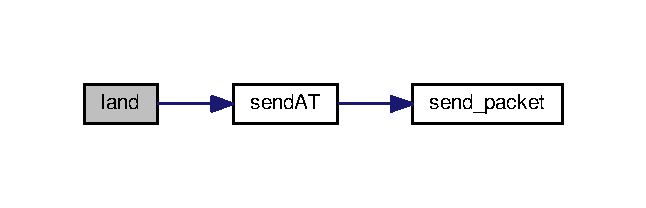
\includegraphics[width=310pt]{group___a_t_commands_ga89c4cd20c1bb10d5624cdcc2154efdd1_cgraph}
\end{center}
\end{figure}




Voici le graphe des appelants de cette fonction \-:\nopagebreak
\begin{figure}[H]
\begin{center}
\leavevmode
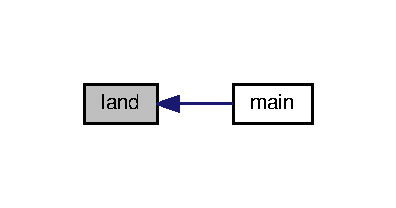
\includegraphics[width=190pt]{group___a_t_commands_ga89c4cd20c1bb10d5624cdcc2154efdd1_icgraph}
\end{center}
\end{figure}


\hypertarget{group___a_t_commands_ga6f1e46bbcb882594c8442c75ae3dedf8}{\index{A\-T\-Commands@{A\-T\-Commands}!new\-A\-R\-Drone@{new\-A\-R\-Drone}}
\index{new\-A\-R\-Drone@{new\-A\-R\-Drone}!ATCommands@{A\-T\-Commands}}
\subsubsection[{new\-A\-R\-Drone}]{\setlength{\rightskip}{0pt plus 5cm}far {\bf ardrone} $\ast$ new\-A\-R\-Drone (
\begin{DoxyParamCaption}
\item[{void}]{}
\end{DoxyParamCaption}
)}}\label{group___a_t_commands_ga6f1e46bbcb882594c8442c75ae3dedf8}


Constructeur de l'objet ardrone. 

\begin{DoxyReturn}{Renvoie}
Handle sur drone 
\end{DoxyReturn}
\begin{DoxyAuthor}{Auteur}
Baudouin Feildel 
\end{DoxyAuthor}


Définition à la ligne 1012 du fichier connexion.\-c.



Voici le graphe des appelants de cette fonction \-:\nopagebreak
\begin{figure}[H]
\begin{center}
\leavevmode
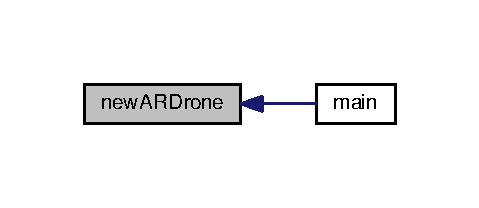
\includegraphics[width=230pt]{group___a_t_commands_ga6f1e46bbcb882594c8442c75ae3dedf8_icgraph}
\end{center}
\end{figure}


\hypertarget{group___a_t_commands_gad4a88a78f2b094bcce69b749a845e11c}{\index{A\-T\-Commands@{A\-T\-Commands}!send\-A\-T@{send\-A\-T}}
\index{send\-A\-T@{send\-A\-T}!ATCommands@{A\-T\-Commands}}
\subsubsection[{send\-A\-T}]{\setlength{\rightskip}{0pt plus 5cm}{\bf cppbool} send\-A\-T (
\begin{DoxyParamCaption}
\item[{far {\bf ardrone} $\ast$}]{dr}
\end{DoxyParamCaption}
)}}\label{group___a_t_commands_gad4a88a78f2b094bcce69b749a845e11c}


Envoyer la commande A\-T qui est dans le buffer du drone dr. 


\begin{DoxyParams}{Paramètres}
{\em far} & ardrone$\ast$ dr \-: Handle du drone \\
\hline
\end{DoxyParams}
\begin{DoxyReturn}{Renvoie}
true \-: buffer envoyé ; false buffer non-\/envoyé 
\end{DoxyReturn}
\begin{DoxyAuthor}{Auteur}
Baudouin Feildel 
\end{DoxyAuthor}


Définition à la ligne 925 du fichier connexion.\-c.



Voici le graphe d'appel pour cette fonction \-:\nopagebreak
\begin{figure}[H]
\begin{center}
\leavevmode
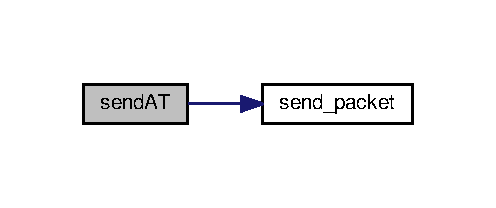
\includegraphics[width=238pt]{group___a_t_commands_gad4a88a78f2b094bcce69b749a845e11c_cgraph}
\end{center}
\end{figure}




Voici le graphe des appelants de cette fonction \-:\nopagebreak
\begin{figure}[H]
\begin{center}
\leavevmode
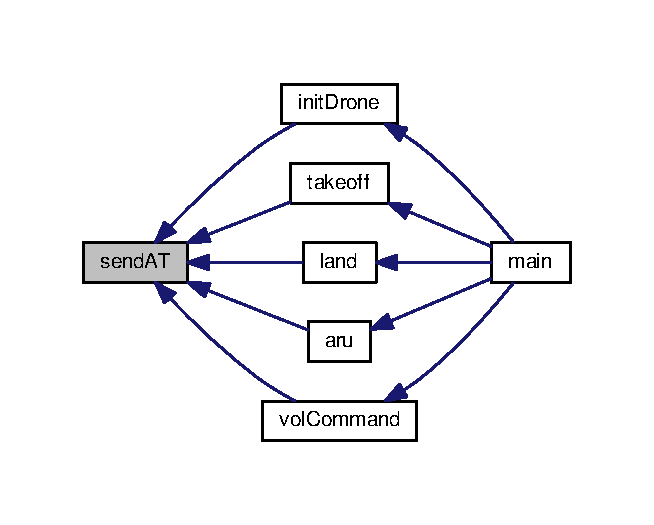
\includegraphics[width=314pt]{group___a_t_commands_gad4a88a78f2b094bcce69b749a845e11c_icgraph}
\end{center}
\end{figure}


\hypertarget{group___a_t_commands_ga9d9aece95d737ed64ba8e9131ff0065c}{\index{A\-T\-Commands@{A\-T\-Commands}!set\-Go\-Up\-Down@{set\-Go\-Up\-Down}}
\index{set\-Go\-Up\-Down@{set\-Go\-Up\-Down}!ATCommands@{A\-T\-Commands}}
\subsubsection[{set\-Go\-Up\-Down}]{\setlength{\rightskip}{0pt plus 5cm}void set\-Go\-Up\-Down (
\begin{DoxyParamCaption}
\item[{far {\bf ardrone} $\ast$}]{dr, }
\item[{float}]{val}
\end{DoxyParamCaption}
)}}\label{group___a_t_commands_ga9d9aece95d737ed64ba8e9131ff0065c}


Mettre une valeur de manière sécurisée dans le buffer de la vitesse verticale du drone dr. 


\begin{DoxyParams}{Paramètres}
{\em far} & ardrone$\ast$ dr \-: Handle du drone \\
\hline
{\em float} & val \-: valeur à inserer \\
\hline
\end{DoxyParams}
\begin{DoxyAuthor}{Auteur}
Baudouin Feildel 
\end{DoxyAuthor}


Définition à la ligne 311 du fichier connexion.\-c.



Voici le graphe des appelants de cette fonction \-:\nopagebreak
\begin{figure}[H]
\begin{center}
\leavevmode
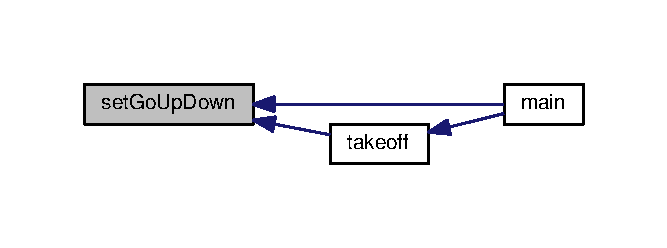
\includegraphics[width=320pt]{group___a_t_commands_ga9d9aece95d737ed64ba8e9131ff0065c_icgraph}
\end{center}
\end{figure}


\hypertarget{group___a_t_commands_ga9a290eee046f983fc53d282c0bc53aff}{\index{A\-T\-Commands@{A\-T\-Commands}!set\-Tilt\-Front\-Back@{set\-Tilt\-Front\-Back}}
\index{set\-Tilt\-Front\-Back@{set\-Tilt\-Front\-Back}!ATCommands@{A\-T\-Commands}}
\subsubsection[{set\-Tilt\-Front\-Back}]{\setlength{\rightskip}{0pt plus 5cm}void set\-Tilt\-Front\-Back (
\begin{DoxyParamCaption}
\item[{far {\bf ardrone} $\ast$}]{dr, }
\item[{float}]{val}
\end{DoxyParamCaption}
)}}\label{group___a_t_commands_ga9a290eee046f983fc53d282c0bc53aff}


Mettre une valeur de manière sécurisé dans le buffer de l'inclinaison avant/arrière du drone dr. 


\begin{DoxyParams}{Paramètres}
{\em far} & ardrone$\ast$ dr \-: Handle du drone \\
\hline
{\em float} & val \-: valeur à insérer \\
\hline
\end{DoxyParams}
\begin{DoxyAuthor}{Auteur}
Baudouin Feildel 
\end{DoxyAuthor}


Définition à la ligne 329 du fichier connexion.\-c.



Voici le graphe des appelants de cette fonction \-:\nopagebreak
\begin{figure}[H]
\begin{center}
\leavevmode
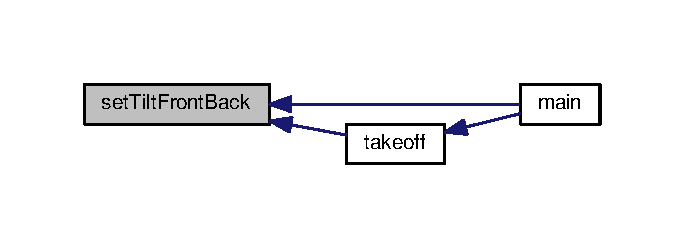
\includegraphics[width=328pt]{group___a_t_commands_ga9a290eee046f983fc53d282c0bc53aff_icgraph}
\end{center}
\end{figure}


\hypertarget{group___a_t_commands_ga28a6f7458f7dbcdf7068b26236f10e2c}{\index{A\-T\-Commands@{A\-T\-Commands}!set\-Tilt\-Left\-Right@{set\-Tilt\-Left\-Right}}
\index{set\-Tilt\-Left\-Right@{set\-Tilt\-Left\-Right}!ATCommands@{A\-T\-Commands}}
\subsubsection[{set\-Tilt\-Left\-Right}]{\setlength{\rightskip}{0pt plus 5cm}void set\-Tilt\-Left\-Right (
\begin{DoxyParamCaption}
\item[{far {\bf ardrone} $\ast$}]{dr, }
\item[{float}]{val}
\end{DoxyParamCaption}
)}}\label{group___a_t_commands_ga28a6f7458f7dbcdf7068b26236f10e2c}


Mettre une valeur de manière sécurisée dans le buffer de l'inclinaison gauche/droite du drone dr. 


\begin{DoxyParams}{Paramètres}
{\em far} & ardrone$\ast$ dr \-: Handle du drone \\
\hline
{\em float} & val \-: valeur à insérer \\
\hline
\end{DoxyParams}
\begin{DoxyAuthor}{Auteur}
Baudouin Feildel 
\end{DoxyAuthor}


Définition à la ligne 338 du fichier connexion.\-c.



Voici le graphe des appelants de cette fonction \-:\nopagebreak
\begin{figure}[H]
\begin{center}
\leavevmode
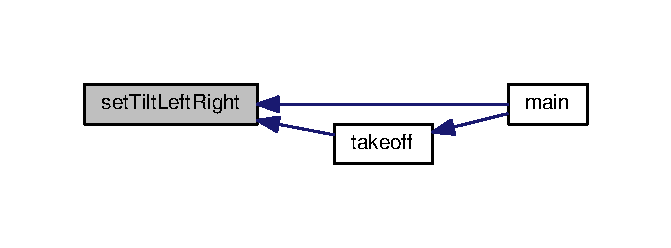
\includegraphics[width=322pt]{group___a_t_commands_ga28a6f7458f7dbcdf7068b26236f10e2c_icgraph}
\end{center}
\end{figure}


\hypertarget{group___a_t_commands_ga0d757863caf7f9c4110ab6e71cac1a4c}{\index{A\-T\-Commands@{A\-T\-Commands}!set\-Turn\-Left\-Right@{set\-Turn\-Left\-Right}}
\index{set\-Turn\-Left\-Right@{set\-Turn\-Left\-Right}!ATCommands@{A\-T\-Commands}}
\subsubsection[{set\-Turn\-Left\-Right}]{\setlength{\rightskip}{0pt plus 5cm}void set\-Turn\-Left\-Right (
\begin{DoxyParamCaption}
\item[{far {\bf ardrone} $\ast$}]{dr, }
\item[{float}]{val}
\end{DoxyParamCaption}
)}}\label{group___a_t_commands_ga0d757863caf7f9c4110ab6e71cac1a4c}


Mettre une valeur dans de manière sécurisée dans le buffer de la vitesse angulaire du drone dr. 


\begin{DoxyParams}{Paramètres}
{\em far} & ardrone$\ast$ dr\-: Handle du drone \\
\hline
{\em float} & val \-: valeur à insérer \\
\hline
\end{DoxyParams}
\begin{DoxyAuthor}{Auteur}
Baudouin Feildel 
\end{DoxyAuthor}


Définition à la ligne 320 du fichier connexion.\-c.



Voici le graphe des appelants de cette fonction \-:\nopagebreak
\begin{figure}[H]
\begin{center}
\leavevmode
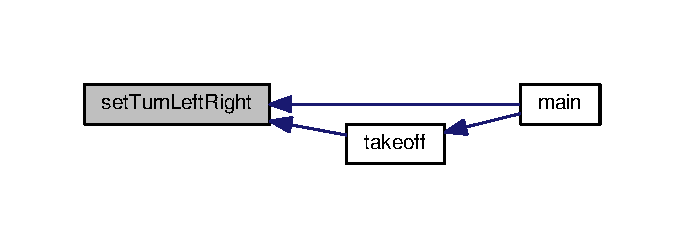
\includegraphics[width=328pt]{group___a_t_commands_ga0d757863caf7f9c4110ab6e71cac1a4c_icgraph}
\end{center}
\end{figure}


\hypertarget{group___a_t_commands_ga565736370f76ee54efe74f65acb3ccc4}{\index{A\-T\-Commands@{A\-T\-Commands}!takeoff@{takeoff}}
\index{takeoff@{takeoff}!ATCommands@{A\-T\-Commands}}
\subsubsection[{takeoff}]{\setlength{\rightskip}{0pt plus 5cm}{\bf cppbool} takeoff (
\begin{DoxyParamCaption}
\item[{far {\bf ardrone} $\ast$}]{dr}
\end{DoxyParamCaption}
)}}\label{group___a_t_commands_ga565736370f76ee54efe74f65acb3ccc4}


Commande le décollage du drone dr. 


\begin{DoxyParams}{Paramètres}
{\em far} & ardrone$\ast$ dr \-: Handle du drone \\
\hline
\end{DoxyParams}
\begin{DoxyReturn}{Renvoie}
true \-: commande envoyée ; false \-: commande non-\/envoyée 
\end{DoxyReturn}
\begin{DoxyAuthor}{Auteur}
Baudouin Feildel 
\end{DoxyAuthor}


Définition à la ligne 957 du fichier connexion.\-c.



Voici le graphe d'appel pour cette fonction \-:\nopagebreak
\begin{figure}[H]
\begin{center}
\leavevmode
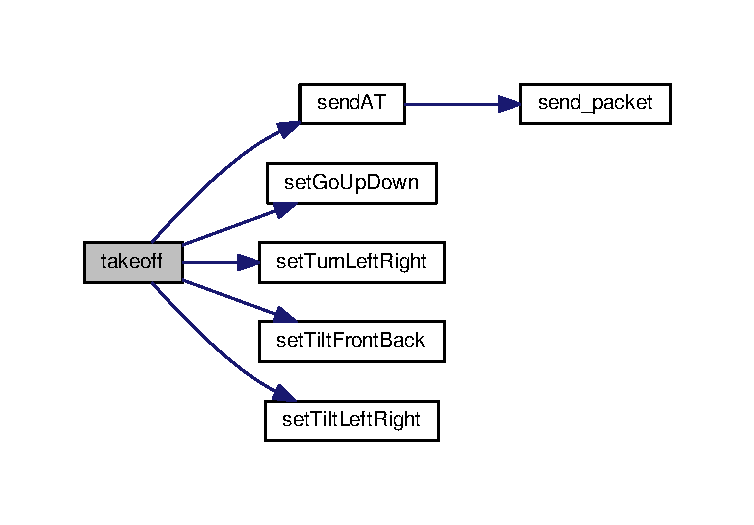
\includegraphics[width=350pt]{group___a_t_commands_ga565736370f76ee54efe74f65acb3ccc4_cgraph}
\end{center}
\end{figure}




Voici le graphe des appelants de cette fonction \-:\nopagebreak
\begin{figure}[H]
\begin{center}
\leavevmode
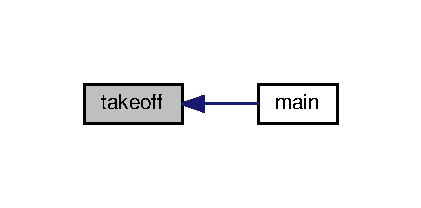
\includegraphics[width=202pt]{group___a_t_commands_ga565736370f76ee54efe74f65acb3ccc4_icgraph}
\end{center}
\end{figure}


\hypertarget{group___a_t_commands_gafba5305bd996ecb4332a17cf68e79928}{\index{A\-T\-Commands@{A\-T\-Commands}!vol\-Command@{vol\-Command}}
\index{vol\-Command@{vol\-Command}!ATCommands@{A\-T\-Commands}}
\subsubsection[{vol\-Command}]{\setlength{\rightskip}{0pt plus 5cm}{\bf cppbool} vol\-Command (
\begin{DoxyParamCaption}
\item[{far {\bf ardrone} $\ast$}]{dr, }
\item[{float}]{tilt\-Left\-Irght\-\_\-, }
\item[{float}]{tilt\-Front\-Back\-\_\-, }
\item[{float}]{go\-Up\-Down\-\_\-, }
\item[{float}]{turn\-Left\-Right\-\_\-}
\end{DoxyParamCaption}
)}}\label{group___a_t_commands_gafba5305bd996ecb4332a17cf68e79928}


Envoi de la commande de vol au drone dr. 


\begin{DoxyParams}{Paramètres}
{\em far} & ardrone$\ast$ dr \-: Handle du drone \\
\hline
{\em float} & tilt\-Left\-Right \-: commande l'inclinaison avant/arrière du drone \\
\hline
{\em float} & tilt\-Front\-Back \-: commande l'inclinaison gauche/droite du drone \\
\hline
{\em float} & go\-Up\-Down \-: commande vitesse verticale du drone \\
\hline
{\em float} & turn\-Left\-Right \-: commande vitesse angulaire du drone \\
\hline
\end{DoxyParams}
\begin{DoxyReturn}{Renvoie}
true \-: commande envoyée ; false \-: commande non-\/envoyée 
\end{DoxyReturn}
\begin{DoxyAuthor}{Auteur}
Baudouin Feildel 
\end{DoxyAuthor}


Définition à la ligne 999 du fichier connexion.\-c.



Voici le graphe d'appel pour cette fonction \-:\nopagebreak
\begin{figure}[H]
\begin{center}
\leavevmode
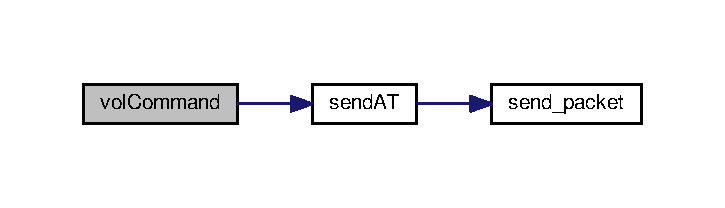
\includegraphics[width=348pt]{group___a_t_commands_gafba5305bd996ecb4332a17cf68e79928_cgraph}
\end{center}
\end{figure}




Voici le graphe des appelants de cette fonction \-:\nopagebreak
\begin{figure}[H]
\begin{center}
\leavevmode
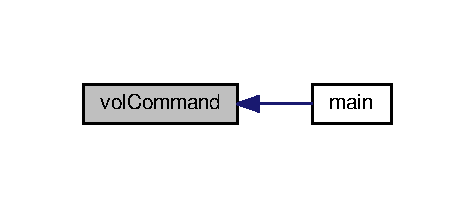
\includegraphics[width=228pt]{group___a_t_commands_gafba5305bd996ecb4332a17cf68e79928_icgraph}
\end{center}
\end{figure}



\chapter{Documentation des espaces de nommage}
\hypertarget{namespace_ui}{\section{Référence de l'espace de nommage Ui}
\label{namespace_ui}\index{Ui@{Ui}}
}

\chapter{Documentation des structures de données}
\hypertarget{structardrone}{\section{Référence de la structure ardrone}
\label{structardrone}\index{ardrone@{ardrone}}
}


Graphe de collaboration de ardrone\-:\nopagebreak
\begin{figure}[H]
\begin{center}
\leavevmode
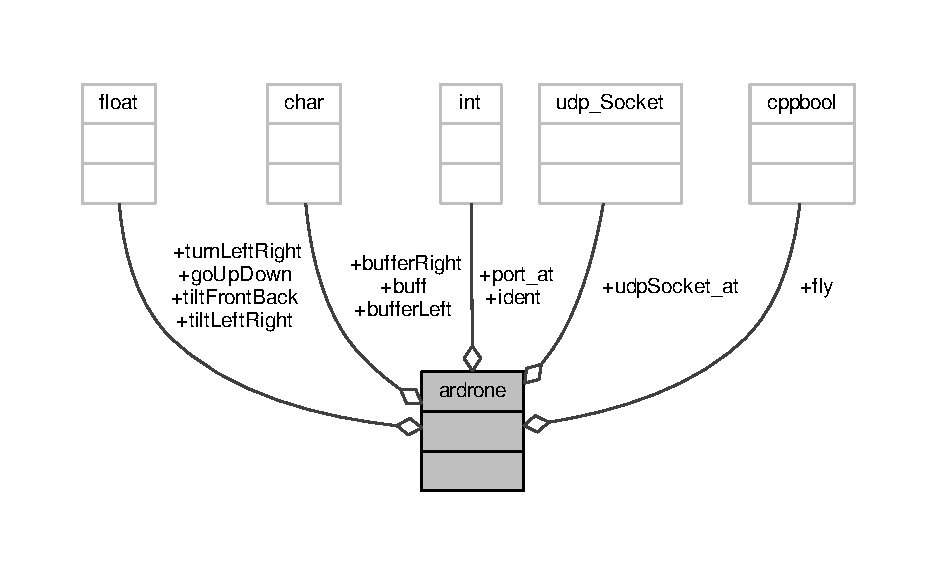
\includegraphics[width=350pt]{structardrone__coll__graph}
\end{center}
\end{figure}
\subsection*{Champs de données}
\begin{DoxyCompactItemize}
\item 
char \hyperlink{structardrone_a825d10649a532df1970c816b4070c690}{buff} \mbox{[}1025\mbox{]}
\item 
udp\-\_\-\-Socket \hyperlink{structardrone_acb3a788ee7164c5350b4bfd7d8312772}{udp\-Socket\-\_\-at}
\item 
int \hyperlink{structardrone_a57f99d232635ffded0d59ea9475639a2}{port\-\_\-at}
\item 
char \hyperlink{structardrone_a800e0449117874d9d1ff10965cdd346f}{buffer\-Left} \mbox{[}20\mbox{]}
\item 
char \hyperlink{structardrone_adcadf1aaae5c4a2ab78bed2f4d77346b}{buffer\-Right} \mbox{[}50\mbox{]}
\item 
int \hyperlink{structardrone_a52e7dc3872878f8c40cd3523fed00c80}{ident}
\item 
\hyperlink{group___a_t_commands_ga58b930fb43c5cd2fc89a84647e6fe51c}{cppbool} \hyperlink{structardrone_a9d1fad21c1121fc07e7f54ae86754cac}{fly}
\item 
float \hyperlink{structardrone_a97a469c16f6798fa7e85ad88a725bdaa}{tilt\-Front\-Back}
\item 
float \hyperlink{structardrone_ae7202985f7f7b5088481dff26f52e319}{tilt\-Left\-Right}
\item 
float \hyperlink{structardrone_a0aeff16c8eb63da12be0a1b57bc10487}{go\-Up\-Down}
\item 
float \hyperlink{structardrone_ad2830725ca67f509c4dd63caf152e8f6}{turn\-Left\-Right}
\end{DoxyCompactItemize}


\subsection{Description détaillée}


Définition à la ligne 231 du fichier connexion.\-c.



\subsection{Documentation des champs}
\hypertarget{structardrone_a825d10649a532df1970c816b4070c690}{\index{ardrone@{ardrone}!buff@{buff}}
\index{buff@{buff}!ardrone@{ardrone}}
\subsubsection[{buff}]{\setlength{\rightskip}{0pt plus 5cm}char buff\mbox{[}1025\mbox{]}}}\label{structardrone_a825d10649a532df1970c816b4070c690}


Définition à la ligne 233 du fichier connexion.\-c.

\hypertarget{structardrone_a800e0449117874d9d1ff10965cdd346f}{\index{ardrone@{ardrone}!buffer\-Left@{buffer\-Left}}
\index{buffer\-Left@{buffer\-Left}!ardrone@{ardrone}}
\subsubsection[{buffer\-Left}]{\setlength{\rightskip}{0pt plus 5cm}char buffer\-Left\mbox{[}20\mbox{]}}}\label{structardrone_a800e0449117874d9d1ff10965cdd346f}


Définition à la ligne 236 du fichier connexion.\-c.

\hypertarget{structardrone_adcadf1aaae5c4a2ab78bed2f4d77346b}{\index{ardrone@{ardrone}!buffer\-Right@{buffer\-Right}}
\index{buffer\-Right@{buffer\-Right}!ardrone@{ardrone}}
\subsubsection[{buffer\-Right}]{\setlength{\rightskip}{0pt plus 5cm}char buffer\-Right\mbox{[}50\mbox{]}}}\label{structardrone_adcadf1aaae5c4a2ab78bed2f4d77346b}


Définition à la ligne 237 du fichier connexion.\-c.

\hypertarget{structardrone_a9d1fad21c1121fc07e7f54ae86754cac}{\index{ardrone@{ardrone}!fly@{fly}}
\index{fly@{fly}!ardrone@{ardrone}}
\subsubsection[{fly}]{\setlength{\rightskip}{0pt plus 5cm}{\bf cppbool} fly}}\label{structardrone_a9d1fad21c1121fc07e7f54ae86754cac}


Définition à la ligne 239 du fichier connexion.\-c.

\hypertarget{structardrone_a0aeff16c8eb63da12be0a1b57bc10487}{\index{ardrone@{ardrone}!go\-Up\-Down@{go\-Up\-Down}}
\index{go\-Up\-Down@{go\-Up\-Down}!ardrone@{ardrone}}
\subsubsection[{go\-Up\-Down}]{\setlength{\rightskip}{0pt plus 5cm}float go\-Up\-Down}}\label{structardrone_a0aeff16c8eb63da12be0a1b57bc10487}


Définition à la ligne 242 du fichier connexion.\-c.

\hypertarget{structardrone_a52e7dc3872878f8c40cd3523fed00c80}{\index{ardrone@{ardrone}!ident@{ident}}
\index{ident@{ident}!ardrone@{ardrone}}
\subsubsection[{ident}]{\setlength{\rightskip}{0pt plus 5cm}int ident}}\label{structardrone_a52e7dc3872878f8c40cd3523fed00c80}


Définition à la ligne 238 du fichier connexion.\-c.

\hypertarget{structardrone_a57f99d232635ffded0d59ea9475639a2}{\index{ardrone@{ardrone}!port\-\_\-at@{port\-\_\-at}}
\index{port\-\_\-at@{port\-\_\-at}!ardrone@{ardrone}}
\subsubsection[{port\-\_\-at}]{\setlength{\rightskip}{0pt plus 5cm}int port\-\_\-at}}\label{structardrone_a57f99d232635ffded0d59ea9475639a2}


Définition à la ligne 235 du fichier connexion.\-c.

\hypertarget{structardrone_a97a469c16f6798fa7e85ad88a725bdaa}{\index{ardrone@{ardrone}!tilt\-Front\-Back@{tilt\-Front\-Back}}
\index{tilt\-Front\-Back@{tilt\-Front\-Back}!ardrone@{ardrone}}
\subsubsection[{tilt\-Front\-Back}]{\setlength{\rightskip}{0pt plus 5cm}float tilt\-Front\-Back}}\label{structardrone_a97a469c16f6798fa7e85ad88a725bdaa}


Définition à la ligne 240 du fichier connexion.\-c.

\hypertarget{structardrone_ae7202985f7f7b5088481dff26f52e319}{\index{ardrone@{ardrone}!tilt\-Left\-Right@{tilt\-Left\-Right}}
\index{tilt\-Left\-Right@{tilt\-Left\-Right}!ardrone@{ardrone}}
\subsubsection[{tilt\-Left\-Right}]{\setlength{\rightskip}{0pt plus 5cm}float tilt\-Left\-Right}}\label{structardrone_ae7202985f7f7b5088481dff26f52e319}


Définition à la ligne 241 du fichier connexion.\-c.

\hypertarget{structardrone_ad2830725ca67f509c4dd63caf152e8f6}{\index{ardrone@{ardrone}!turn\-Left\-Right@{turn\-Left\-Right}}
\index{turn\-Left\-Right@{turn\-Left\-Right}!ardrone@{ardrone}}
\subsubsection[{turn\-Left\-Right}]{\setlength{\rightskip}{0pt plus 5cm}float turn\-Left\-Right}}\label{structardrone_ad2830725ca67f509c4dd63caf152e8f6}


Définition à la ligne 243 du fichier connexion.\-c.

\hypertarget{structardrone_acb3a788ee7164c5350b4bfd7d8312772}{\index{ardrone@{ardrone}!udp\-Socket\-\_\-at@{udp\-Socket\-\_\-at}}
\index{udp\-Socket\-\_\-at@{udp\-Socket\-\_\-at}!ardrone@{ardrone}}
\subsubsection[{udp\-Socket\-\_\-at}]{\setlength{\rightskip}{0pt plus 5cm}udp\-\_\-\-Socket udp\-Socket\-\_\-at}}\label{structardrone_acb3a788ee7164c5350b4bfd7d8312772}


Définition à la ligne 234 du fichier connexion.\-c.



La documentation de cette structure a été générée à partir du fichier suivant \-:\begin{DoxyCompactItemize}
\item 
/media/\-D\-E\-V\-E\-L/\-Projet\-I\-U\-T/\-Drone\-Wifi/sources/wifi/\hyperlink{connexion_8c}{connexion.\-c}\end{DoxyCompactItemize}

\hypertarget{class_a_r_drone}{\section{Référence de la classe A\-R\-Drone}
\label{class_a_r_drone}\index{A\-R\-Drone@{A\-R\-Drone}}
}


{\ttfamily \#include $<$ardrone.\-h$>$}



Graphe d'héritage de A\-R\-Drone\-:
\nopagebreak
\begin{figure}[H]
\begin{center}
\leavevmode
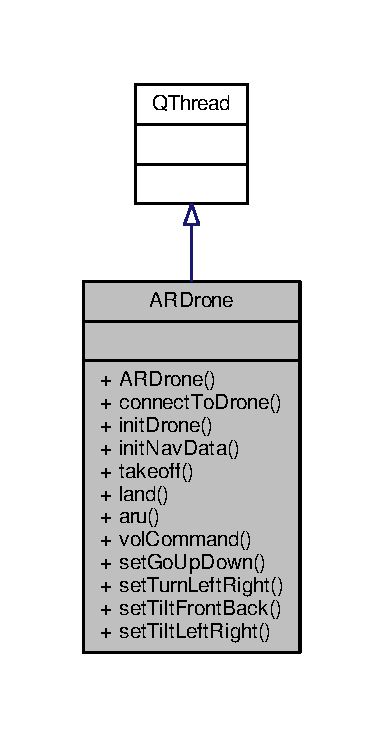
\includegraphics[width=184pt]{class_a_r_drone__inherit__graph}
\end{center}
\end{figure}


Graphe de collaboration de A\-R\-Drone\-:
\nopagebreak
\begin{figure}[H]
\begin{center}
\leavevmode
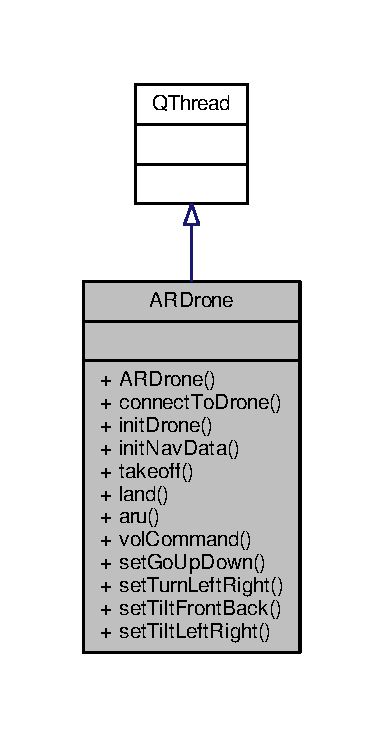
\includegraphics[width=184pt]{class_a_r_drone__coll__graph}
\end{center}
\end{figure}
\subsection*{Fonctions membres publiques}
\begin{DoxyCompactItemize}
\item 
\hyperlink{class_a_r_drone_a9f5df81d1e4b136238e7b89b03cf915b}{A\-R\-Drone} (Q\-Object $\ast$parent=0)
\item 
bool \hyperlink{class_a_r_drone_a0ba4b4e4cf7a107a1587152af3f4fbab}{connect\-To\-Drone} (void)
\begin{DoxyCompactList}\small\item\em Initialise la connexion au drone. \end{DoxyCompactList}\item 
bool \hyperlink{class_a_r_drone_ab447af60c30509710f55922ff07fc3a4}{init\-Drone} (void)
\begin{DoxyCompactList}\small\item\em Initialise le drone (à utiliser avant de lancer la navigation) \end{DoxyCompactList}\item 
bool \hyperlink{class_a_r_drone_a36946b429549afb5b1d64c0ff1fe4fbb}{init\-Nav\-Data} (void)
\begin{DoxyCompactList}\small\item\em Initialise le fux de données. \end{DoxyCompactList}\item 
bool \hyperlink{class_a_r_drone_a34d3e2ff71b9fc05e2faa20015d320c8}{takeoff} (void)
\begin{DoxyCompactList}\small\item\em Demande de décollage. \end{DoxyCompactList}\item 
bool \hyperlink{class_a_r_drone_a4735e9dbf7f8c0c43a6e4f55511d7262}{land} (void)
\begin{DoxyCompactList}\small\item\em Demande d'atterrissage. \end{DoxyCompactList}\item 
bool \hyperlink{class_a_r_drone_ac0bf02a934602af7eb48e20e2717bb3e}{aru} (void)
\begin{DoxyCompactList}\small\item\em Demande d'arrêt d'urgence. \end{DoxyCompactList}\item 
bool \hyperlink{class_a_r_drone_a4a3c6bdd5043578998f074ca7a85d146}{vol\-Command} (float tilt\-Left\-Right\-\_\-, float tilt\-Front\-Back\-\_\-, float go\-Up\-Down\-\_\-, float turn\-Left\-Right\-\_\-)
\begin{DoxyCompactList}\small\item\em Pilotage du drone en vol. \end{DoxyCompactList}\item 
void \hyperlink{class_a_r_drone_a40d5afd3a519061379938368c9096df0}{set\-Go\-Up\-Down} (float val)
\begin{DoxyCompactList}\small\item\em Setter sécurisé de la valeur de la vitesse verticale. \end{DoxyCompactList}\item 
void \hyperlink{class_a_r_drone_a846d9ca708547b77d6353b8c544e2764}{set\-Turn\-Left\-Right} (float val)
\begin{DoxyCompactList}\small\item\em Setter sécurisé de la valeur de la vitesse angulaire. \end{DoxyCompactList}\item 
void \hyperlink{class_a_r_drone_a35091a8252bbb1cffab5c07834d1f263}{set\-Tilt\-Front\-Back} (float val)
\begin{DoxyCompactList}\small\item\em Setter sécurisé de la valeur de l'inclinaison avant arrière. \end{DoxyCompactList}\item 
void \hyperlink{class_a_r_drone_a2cd513a18603d81fdbc8167c103af577}{set\-Tilt\-Left\-Right} (float val)
\begin{DoxyCompactList}\small\item\em Setter sécurisé de la valeur de l'inclinaison gauche droite. \end{DoxyCompactList}\end{DoxyCompactItemize}


\subsection{Description détaillée}


Définition à la ligne 9 du fichier ardrone.\-h.



\subsection{Documentation des constructeurs et destructeur}
\hypertarget{class_a_r_drone_a9f5df81d1e4b136238e7b89b03cf915b}{\index{A\-R\-Drone@{A\-R\-Drone}!A\-R\-Drone@{A\-R\-Drone}}
\index{A\-R\-Drone@{A\-R\-Drone}!ARDrone@{A\-R\-Drone}}
\subsubsection[{A\-R\-Drone}]{\setlength{\rightskip}{0pt plus 5cm}{\bf A\-R\-Drone} (
\begin{DoxyParamCaption}
\item[{Q\-Object $\ast$}]{parent = {\ttfamily 0}}
\end{DoxyParamCaption}
)\hspace{0.3cm}{\ttfamily [explicit]}}}\label{class_a_r_drone_a9f5df81d1e4b136238e7b89b03cf915b}


Définition à la ligne 3 du fichier ardrone.\-cpp.



\subsection{Documentation des fonctions membres}
\hypertarget{class_a_r_drone_ac0bf02a934602af7eb48e20e2717bb3e}{\index{A\-R\-Drone@{A\-R\-Drone}!aru@{aru}}
\index{aru@{aru}!ARDrone@{A\-R\-Drone}}
\subsubsection[{aru}]{\setlength{\rightskip}{0pt plus 5cm}bool aru (
\begin{DoxyParamCaption}
\item[{void}]{}
\end{DoxyParamCaption}
)}}\label{class_a_r_drone_ac0bf02a934602af7eb48e20e2717bb3e}


Demande d'arrêt d'urgence. 

\begin{DoxyReturn}{Renvoie}
(bool) true \-: demande envoyée ; false \-: demande non-\/envoyée 
\end{DoxyReturn}


Définition à la ligne 111 du fichier ardrone.\-cpp.

\hypertarget{class_a_r_drone_a0ba4b4e4cf7a107a1587152af3f4fbab}{\index{A\-R\-Drone@{A\-R\-Drone}!connect\-To\-Drone@{connect\-To\-Drone}}
\index{connect\-To\-Drone@{connect\-To\-Drone}!ARDrone@{A\-R\-Drone}}
\subsubsection[{connect\-To\-Drone}]{\setlength{\rightskip}{0pt plus 5cm}bool connect\-To\-Drone (
\begin{DoxyParamCaption}
\item[{void}]{}
\end{DoxyParamCaption}
)}}\label{class_a_r_drone_a0ba4b4e4cf7a107a1587152af3f4fbab}


Initialise la connexion au drone. 

\begin{DoxyReturn}{Renvoie}
(bool) true \-: Connexion réussie ; false \-: Connexion échouée 
\end{DoxyReturn}
\begin{DoxyAuthor}{Auteur}
Baudouin Feildel 
\end{DoxyAuthor}


Définition à la ligne 15 du fichier ardrone.\-cpp.



Voici le graphe des appelants de cette fonction \-:
\nopagebreak
\begin{figure}[H]
\begin{center}
\leavevmode
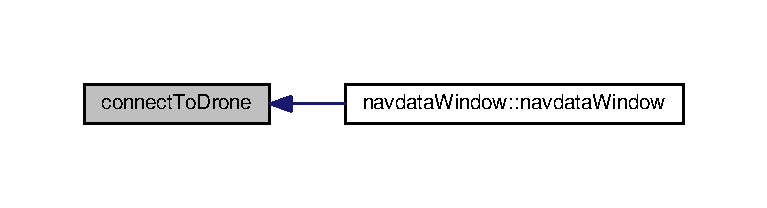
\includegraphics[width=350pt]{class_a_r_drone_a0ba4b4e4cf7a107a1587152af3f4fbab_icgraph}
\end{center}
\end{figure}


\hypertarget{class_a_r_drone_ab447af60c30509710f55922ff07fc3a4}{\index{A\-R\-Drone@{A\-R\-Drone}!init\-Drone@{init\-Drone}}
\index{init\-Drone@{init\-Drone}!ARDrone@{A\-R\-Drone}}
\subsubsection[{init\-Drone}]{\setlength{\rightskip}{0pt plus 5cm}bool init\-Drone (
\begin{DoxyParamCaption}
\item[{void}]{}
\end{DoxyParamCaption}
)}}\label{class_a_r_drone_ab447af60c30509710f55922ff07fc3a4}


Initialise le drone (à utiliser avant de lancer la navigation) 

\begin{DoxyReturn}{Renvoie}
(bool) true \-: Initialisation réussie ; false \-: Initialisation échouée 
\end{DoxyReturn}
\begin{DoxyAuthor}{Auteur}
Baudouin Feildel 
\end{DoxyAuthor}


Définition à la ligne 35 du fichier ardrone.\-cpp.

\hypertarget{class_a_r_drone_a36946b429549afb5b1d64c0ff1fe4fbb}{\index{A\-R\-Drone@{A\-R\-Drone}!init\-Nav\-Data@{init\-Nav\-Data}}
\index{init\-Nav\-Data@{init\-Nav\-Data}!ARDrone@{A\-R\-Drone}}
\subsubsection[{init\-Nav\-Data}]{\setlength{\rightskip}{0pt plus 5cm}bool init\-Nav\-Data (
\begin{DoxyParamCaption}
\item[{void}]{}
\end{DoxyParamCaption}
)}}\label{class_a_r_drone_a36946b429549afb5b1d64c0ff1fe4fbb}


Initialise le fux de données. 

\begin{DoxyReturn}{Renvoie}
(bool) true \-: Initialisation réussie ; false \-: Initialisation échouée 
\end{DoxyReturn}
\begin{DoxyAuthor}{Auteur}
Baudouin Feildel 
\end{DoxyAuthor}


Définition à la ligne 51 du fichier ardrone.\-cpp.



Voici le graphe des appelants de cette fonction \-:
\nopagebreak
\begin{figure}[H]
\begin{center}
\leavevmode
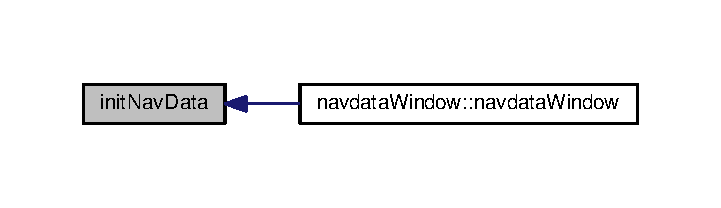
\includegraphics[width=346pt]{class_a_r_drone_a36946b429549afb5b1d64c0ff1fe4fbb_icgraph}
\end{center}
\end{figure}


\hypertarget{class_a_r_drone_a4735e9dbf7f8c0c43a6e4f55511d7262}{\index{A\-R\-Drone@{A\-R\-Drone}!land@{land}}
\index{land@{land}!ARDrone@{A\-R\-Drone}}
\subsubsection[{land}]{\setlength{\rightskip}{0pt plus 5cm}bool land (
\begin{DoxyParamCaption}
\item[{void}]{}
\end{DoxyParamCaption}
)}}\label{class_a_r_drone_a4735e9dbf7f8c0c43a6e4f55511d7262}


Demande d'atterrissage. 

\begin{DoxyReturn}{Renvoie}
(bool) true \-: demande envoyée ; false \-: demande non-\/envoyée 
\end{DoxyReturn}


Définition à la ligne 101 du fichier ardrone.\-cpp.

\hypertarget{class_a_r_drone_a40d5afd3a519061379938368c9096df0}{\index{A\-R\-Drone@{A\-R\-Drone}!set\-Go\-Up\-Down@{set\-Go\-Up\-Down}}
\index{set\-Go\-Up\-Down@{set\-Go\-Up\-Down}!ARDrone@{A\-R\-Drone}}
\subsubsection[{set\-Go\-Up\-Down}]{\setlength{\rightskip}{0pt plus 5cm}void set\-Go\-Up\-Down (
\begin{DoxyParamCaption}
\item[{float}]{val}
\end{DoxyParamCaption}
)\hspace{0.3cm}{\ttfamily [inline]}}}\label{class_a_r_drone_a40d5afd3a519061379938368c9096df0}


Setter sécurisé de la valeur de la vitesse verticale. 


\begin{DoxyParams}{Paramètres}
{\em float} & val \-: valeur à écrire \\
\hline
\end{DoxyParams}
\begin{DoxyAuthor}{Auteur}
Baudouin Feildel 
\end{DoxyAuthor}


Définition à la ligne 79 du fichier ardrone.\-h.



Voici le graphe des appelants de cette fonction \-:
\nopagebreak
\begin{figure}[H]
\begin{center}
\leavevmode
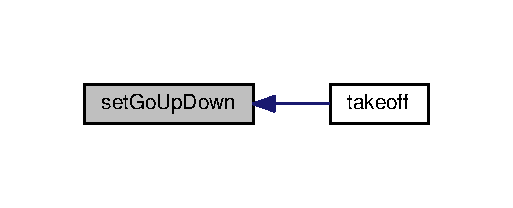
\includegraphics[width=246pt]{class_a_r_drone_a40d5afd3a519061379938368c9096df0_icgraph}
\end{center}
\end{figure}


\hypertarget{class_a_r_drone_a35091a8252bbb1cffab5c07834d1f263}{\index{A\-R\-Drone@{A\-R\-Drone}!set\-Tilt\-Front\-Back@{set\-Tilt\-Front\-Back}}
\index{set\-Tilt\-Front\-Back@{set\-Tilt\-Front\-Back}!ARDrone@{A\-R\-Drone}}
\subsubsection[{set\-Tilt\-Front\-Back}]{\setlength{\rightskip}{0pt plus 5cm}void set\-Tilt\-Front\-Back (
\begin{DoxyParamCaption}
\item[{float}]{val}
\end{DoxyParamCaption}
)\hspace{0.3cm}{\ttfamily [inline]}}}\label{class_a_r_drone_a35091a8252bbb1cffab5c07834d1f263}


Setter sécurisé de la valeur de l'inclinaison avant arrière. 


\begin{DoxyParams}{Paramètres}
{\em float} & val \-: valeur à écrire \\
\hline
\end{DoxyParams}
\begin{DoxyAuthor}{Auteur}
Baudouin Feildel 
\end{DoxyAuthor}


Définition à la ligne 95 du fichier ardrone.\-h.



Voici le graphe des appelants de cette fonction \-:
\nopagebreak
\begin{figure}[H]
\begin{center}
\leavevmode
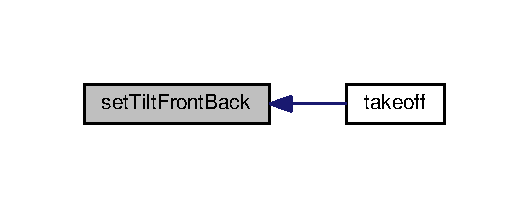
\includegraphics[width=254pt]{class_a_r_drone_a35091a8252bbb1cffab5c07834d1f263_icgraph}
\end{center}
\end{figure}


\hypertarget{class_a_r_drone_a2cd513a18603d81fdbc8167c103af577}{\index{A\-R\-Drone@{A\-R\-Drone}!set\-Tilt\-Left\-Right@{set\-Tilt\-Left\-Right}}
\index{set\-Tilt\-Left\-Right@{set\-Tilt\-Left\-Right}!ARDrone@{A\-R\-Drone}}
\subsubsection[{set\-Tilt\-Left\-Right}]{\setlength{\rightskip}{0pt plus 5cm}void set\-Tilt\-Left\-Right (
\begin{DoxyParamCaption}
\item[{float}]{val}
\end{DoxyParamCaption}
)\hspace{0.3cm}{\ttfamily [inline]}}}\label{class_a_r_drone_a2cd513a18603d81fdbc8167c103af577}


Setter sécurisé de la valeur de l'inclinaison gauche droite. 


\begin{DoxyParams}{Paramètres}
{\em float} & val \-: valeur à écrire \\
\hline
\end{DoxyParams}
\begin{DoxyAuthor}{Auteur}
Baudouin Feildel 
\end{DoxyAuthor}


Définition à la ligne 103 du fichier ardrone.\-h.



Voici le graphe des appelants de cette fonction \-:
\nopagebreak
\begin{figure}[H]
\begin{center}
\leavevmode
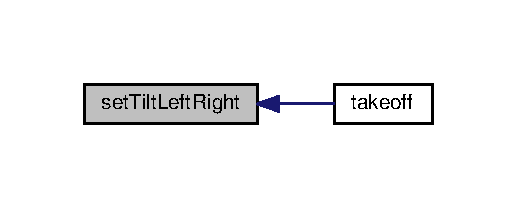
\includegraphics[width=248pt]{class_a_r_drone_a2cd513a18603d81fdbc8167c103af577_icgraph}
\end{center}
\end{figure}


\hypertarget{class_a_r_drone_a846d9ca708547b77d6353b8c544e2764}{\index{A\-R\-Drone@{A\-R\-Drone}!set\-Turn\-Left\-Right@{set\-Turn\-Left\-Right}}
\index{set\-Turn\-Left\-Right@{set\-Turn\-Left\-Right}!ARDrone@{A\-R\-Drone}}
\subsubsection[{set\-Turn\-Left\-Right}]{\setlength{\rightskip}{0pt plus 5cm}void set\-Turn\-Left\-Right (
\begin{DoxyParamCaption}
\item[{float}]{val}
\end{DoxyParamCaption}
)\hspace{0.3cm}{\ttfamily [inline]}}}\label{class_a_r_drone_a846d9ca708547b77d6353b8c544e2764}


Setter sécurisé de la valeur de la vitesse angulaire. 


\begin{DoxyParams}{Paramètres}
{\em float} & val \-: valeur à écrire \\
\hline
\end{DoxyParams}
\begin{DoxyAuthor}{Auteur}
Baudouin Feildel 
\end{DoxyAuthor}


Définition à la ligne 87 du fichier ardrone.\-h.



Voici le graphe des appelants de cette fonction \-:
\nopagebreak
\begin{figure}[H]
\begin{center}
\leavevmode
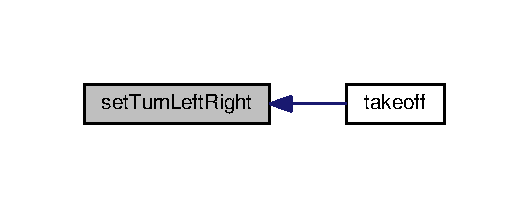
\includegraphics[width=254pt]{class_a_r_drone_a846d9ca708547b77d6353b8c544e2764_icgraph}
\end{center}
\end{figure}


\hypertarget{class_a_r_drone_a34d3e2ff71b9fc05e2faa20015d320c8}{\index{A\-R\-Drone@{A\-R\-Drone}!takeoff@{takeoff}}
\index{takeoff@{takeoff}!ARDrone@{A\-R\-Drone}}
\subsubsection[{takeoff}]{\setlength{\rightskip}{0pt plus 5cm}bool takeoff (
\begin{DoxyParamCaption}
\item[{void}]{}
\end{DoxyParamCaption}
)}}\label{class_a_r_drone_a34d3e2ff71b9fc05e2faa20015d320c8}


Demande de décollage. 

\begin{DoxyReturn}{Renvoie}
(bool) true \-: demande envoyée ; false \-: demande non-\/envoyée 
\end{DoxyReturn}
\begin{DoxyAuthor}{Auteur}
Baudouin Feildel 
\end{DoxyAuthor}


Définition à la ligne 80 du fichier ardrone.\-cpp.



Voici le graphe d'appel pour cette fonction \-:
\nopagebreak
\begin{figure}[H]
\begin{center}
\leavevmode
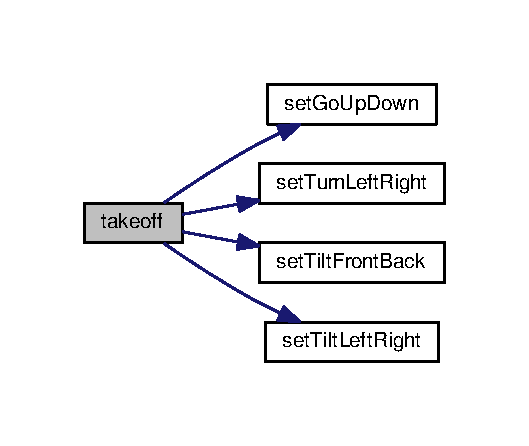
\includegraphics[width=254pt]{class_a_r_drone_a34d3e2ff71b9fc05e2faa20015d320c8_cgraph}
\end{center}
\end{figure}


\hypertarget{class_a_r_drone_a4a3c6bdd5043578998f074ca7a85d146}{\index{A\-R\-Drone@{A\-R\-Drone}!vol\-Command@{vol\-Command}}
\index{vol\-Command@{vol\-Command}!ARDrone@{A\-R\-Drone}}
\subsubsection[{vol\-Command}]{\setlength{\rightskip}{0pt plus 5cm}bool vol\-Command (
\begin{DoxyParamCaption}
\item[{float}]{tilt\-Left\-Right\-\_\-, }
\item[{float}]{tilt\-Front\-Back\-\_\-, }
\item[{float}]{go\-Up\-Down\-\_\-, }
\item[{float}]{turn\-Left\-Right\-\_\-}
\end{DoxyParamCaption}
)}}\label{class_a_r_drone_a4a3c6bdd5043578998f074ca7a85d146}


Pilotage du drone en vol. 


\begin{DoxyParams}{Paramètres}
{\em float} & tilt\-Left\-Right\-\_\- Inclinaison gauche droite ; \mbox{[}-\/1,1\mbox{]} \\
\hline
{\em float} & tilt\-Front\-Back\-\_\- Inclinaison avant arrière ; \mbox{[}-\/1;1\mbox{]} \\
\hline
{\em float} & go\-Up\-Down\-\_\- Vitesse verticale ; \mbox{[}-\/1;1\mbox{]} \\
\hline
{\em float} & turn\-Left\-Right\-\_\- Vitesse angulaire ; \mbox{[}-\/1;1\mbox{]} \\
\hline
\end{DoxyParams}
\begin{DoxyReturn}{Renvoie}
(bool) true \-: commande envoyée ; false \-: commande non-\/envoyée 
\end{DoxyReturn}
\begin{DoxyAuthor}{Auteur}
Baudouin Feildel 
\end{DoxyAuthor}


Définition à la ligne 121 du fichier ardrone.\-cpp.



La documentation de cette classe a été générée à partir des fichiers suivants \-:\begin{DoxyCompactItemize}
\item 
/media/\-D\-E\-V\-E\-L/\-Projet\-I\-U\-T/\-Drone\-Wifi/sources/keyboard\-Command/\hyperlink{ardrone_8h}{ardrone.\-h}\item 
/media/\-D\-E\-V\-E\-L/\-Projet\-I\-U\-T/\-Drone\-Wifi/sources/keyboard\-Command/\hyperlink{ardrone_8cpp}{ardrone.\-cpp}\end{DoxyCompactItemize}

\hypertarget{structetat__commandes}{\section{Référence de la structure etat\-\_\-commandes}
\label{structetat__commandes}\index{etat\-\_\-commandes@{etat\-\_\-commandes}}
}


Graphe de collaboration de etat\-\_\-commandes\-:\nopagebreak
\begin{figure}[H]
\begin{center}
\leavevmode
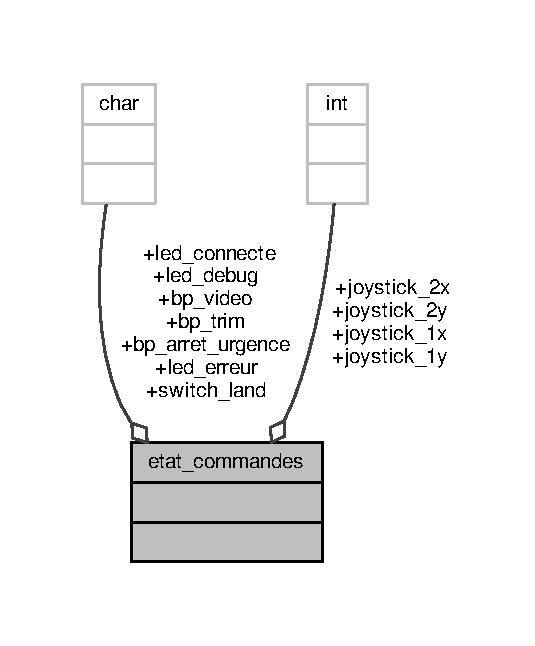
\includegraphics[width=257pt]{structetat__commandes__coll__graph}
\end{center}
\end{figure}
\subsection*{Champs de données}
\begin{DoxyCompactItemize}
\item 
char \hyperlink{structetat__commandes_a38345f0aebb4de891510939a4d1b6d3f}{led\-\_\-connecte}
\item 
char \hyperlink{structetat__commandes_a3aaef46c6ca19a2afb10c86c5300d067}{led\-\_\-erreur}
\item 
char \hyperlink{structetat__commandes_aa6c5f40a4dec71b510d913e4c09e3cee}{led\-\_\-debug}
\item 
char \hyperlink{structetat__commandes_adcce0767b69b6aa61d9815c90afece60}{bp\-\_\-arret\-\_\-urgence}
\item 
char \hyperlink{structetat__commandes_a9f65380fb32037e5147720cbd1c20cad}{bp\-\_\-video}
\item 
char \hyperlink{structetat__commandes_adc9e1c40950878e4b174300aef5c8628}{bp\-\_\-trim}
\item 
char \hyperlink{structetat__commandes_af0fce6b96a884e05a43ec95b76d1f6db}{switch\-\_\-land}
\item 
int \hyperlink{structetat__commandes_aefd8dcb52ec6c8b5014e4e4a07ce36f5}{joystick\-\_\-1x}
\item 
int \hyperlink{structetat__commandes_a44464264b58e816437b75338c8071db7}{joystick\-\_\-1y}
\item 
int \hyperlink{structetat__commandes_ab13efe455d7039d936ed7c8909581001}{joystick\-\_\-2x}
\item 
int \hyperlink{structetat__commandes_a22286f59a64543f8e90ee521270110bd}{joystick\-\_\-2y}
\end{DoxyCompactItemize}


\subsection{Description détaillée}


Définition à la ligne 58 du fichier connexion.\-c.



\subsection{Documentation des champs}
\hypertarget{structetat__commandes_adcce0767b69b6aa61d9815c90afece60}{\index{etat\-\_\-commandes@{etat\-\_\-commandes}!bp\-\_\-arret\-\_\-urgence@{bp\-\_\-arret\-\_\-urgence}}
\index{bp\-\_\-arret\-\_\-urgence@{bp\-\_\-arret\-\_\-urgence}!etat_commandes@{etat\-\_\-commandes}}
\subsubsection[{bp\-\_\-arret\-\_\-urgence}]{\setlength{\rightskip}{0pt plus 5cm}char bp\-\_\-arret\-\_\-urgence}}\label{structetat__commandes_adcce0767b69b6aa61d9815c90afece60}


Définition à la ligne 65 du fichier connexion.\-c.

\hypertarget{structetat__commandes_adc9e1c40950878e4b174300aef5c8628}{\index{etat\-\_\-commandes@{etat\-\_\-commandes}!bp\-\_\-trim@{bp\-\_\-trim}}
\index{bp\-\_\-trim@{bp\-\_\-trim}!etat_commandes@{etat\-\_\-commandes}}
\subsubsection[{bp\-\_\-trim}]{\setlength{\rightskip}{0pt plus 5cm}char bp\-\_\-trim}}\label{structetat__commandes_adc9e1c40950878e4b174300aef5c8628}


Définition à la ligne 67 du fichier connexion.\-c.

\hypertarget{structetat__commandes_a9f65380fb32037e5147720cbd1c20cad}{\index{etat\-\_\-commandes@{etat\-\_\-commandes}!bp\-\_\-video@{bp\-\_\-video}}
\index{bp\-\_\-video@{bp\-\_\-video}!etat_commandes@{etat\-\_\-commandes}}
\subsubsection[{bp\-\_\-video}]{\setlength{\rightskip}{0pt plus 5cm}char bp\-\_\-video}}\label{structetat__commandes_a9f65380fb32037e5147720cbd1c20cad}


Définition à la ligne 66 du fichier connexion.\-c.

\hypertarget{structetat__commandes_aefd8dcb52ec6c8b5014e4e4a07ce36f5}{\index{etat\-\_\-commandes@{etat\-\_\-commandes}!joystick\-\_\-1x@{joystick\-\_\-1x}}
\index{joystick\-\_\-1x@{joystick\-\_\-1x}!etat_commandes@{etat\-\_\-commandes}}
\subsubsection[{joystick\-\_\-1x}]{\setlength{\rightskip}{0pt plus 5cm}int joystick\-\_\-1x}}\label{structetat__commandes_aefd8dcb52ec6c8b5014e4e4a07ce36f5}


Définition à la ligne 70 du fichier connexion.\-c.

\hypertarget{structetat__commandes_a44464264b58e816437b75338c8071db7}{\index{etat\-\_\-commandes@{etat\-\_\-commandes}!joystick\-\_\-1y@{joystick\-\_\-1y}}
\index{joystick\-\_\-1y@{joystick\-\_\-1y}!etat_commandes@{etat\-\_\-commandes}}
\subsubsection[{joystick\-\_\-1y}]{\setlength{\rightskip}{0pt plus 5cm}int joystick\-\_\-1y}}\label{structetat__commandes_a44464264b58e816437b75338c8071db7}


Définition à la ligne 71 du fichier connexion.\-c.

\hypertarget{structetat__commandes_ab13efe455d7039d936ed7c8909581001}{\index{etat\-\_\-commandes@{etat\-\_\-commandes}!joystick\-\_\-2x@{joystick\-\_\-2x}}
\index{joystick\-\_\-2x@{joystick\-\_\-2x}!etat_commandes@{etat\-\_\-commandes}}
\subsubsection[{joystick\-\_\-2x}]{\setlength{\rightskip}{0pt plus 5cm}int joystick\-\_\-2x}}\label{structetat__commandes_ab13efe455d7039d936ed7c8909581001}


Définition à la ligne 72 du fichier connexion.\-c.

\hypertarget{structetat__commandes_a22286f59a64543f8e90ee521270110bd}{\index{etat\-\_\-commandes@{etat\-\_\-commandes}!joystick\-\_\-2y@{joystick\-\_\-2y}}
\index{joystick\-\_\-2y@{joystick\-\_\-2y}!etat_commandes@{etat\-\_\-commandes}}
\subsubsection[{joystick\-\_\-2y}]{\setlength{\rightskip}{0pt plus 5cm}int joystick\-\_\-2y}}\label{structetat__commandes_a22286f59a64543f8e90ee521270110bd}


Définition à la ligne 73 du fichier connexion.\-c.

\hypertarget{structetat__commandes_a38345f0aebb4de891510939a4d1b6d3f}{\index{etat\-\_\-commandes@{etat\-\_\-commandes}!led\-\_\-connecte@{led\-\_\-connecte}}
\index{led\-\_\-connecte@{led\-\_\-connecte}!etat_commandes@{etat\-\_\-commandes}}
\subsubsection[{led\-\_\-connecte}]{\setlength{\rightskip}{0pt plus 5cm}char led\-\_\-connecte}}\label{structetat__commandes_a38345f0aebb4de891510939a4d1b6d3f}


Définition à la ligne 61 du fichier connexion.\-c.

\hypertarget{structetat__commandes_aa6c5f40a4dec71b510d913e4c09e3cee}{\index{etat\-\_\-commandes@{etat\-\_\-commandes}!led\-\_\-debug@{led\-\_\-debug}}
\index{led\-\_\-debug@{led\-\_\-debug}!etat_commandes@{etat\-\_\-commandes}}
\subsubsection[{led\-\_\-debug}]{\setlength{\rightskip}{0pt plus 5cm}char led\-\_\-debug}}\label{structetat__commandes_aa6c5f40a4dec71b510d913e4c09e3cee}


Définition à la ligne 63 du fichier connexion.\-c.

\hypertarget{structetat__commandes_a3aaef46c6ca19a2afb10c86c5300d067}{\index{etat\-\_\-commandes@{etat\-\_\-commandes}!led\-\_\-erreur@{led\-\_\-erreur}}
\index{led\-\_\-erreur@{led\-\_\-erreur}!etat_commandes@{etat\-\_\-commandes}}
\subsubsection[{led\-\_\-erreur}]{\setlength{\rightskip}{0pt plus 5cm}char led\-\_\-erreur}}\label{structetat__commandes_a3aaef46c6ca19a2afb10c86c5300d067}


Définition à la ligne 62 du fichier connexion.\-c.

\hypertarget{structetat__commandes_af0fce6b96a884e05a43ec95b76d1f6db}{\index{etat\-\_\-commandes@{etat\-\_\-commandes}!switch\-\_\-land@{switch\-\_\-land}}
\index{switch\-\_\-land@{switch\-\_\-land}!etat_commandes@{etat\-\_\-commandes}}
\subsubsection[{switch\-\_\-land}]{\setlength{\rightskip}{0pt plus 5cm}char switch\-\_\-land}}\label{structetat__commandes_af0fce6b96a884e05a43ec95b76d1f6db}


Définition à la ligne 68 du fichier connexion.\-c.



La documentation de cette structure a été générée à partir du fichier suivant \-:\begin{DoxyCompactItemize}
\item 
/media/\-D\-E\-V\-E\-L/\-Projet\-I\-U\-T/\-Drone\-Wifi/sources/wifi/\hyperlink{connexion_8c}{connexion.\-c}\end{DoxyCompactItemize}

\hypertarget{class_main_window}{\section{Référence de la classe Main\-Window}
\label{class_main_window}\index{Main\-Window@{Main\-Window}}
}


{\ttfamily \#include $<$mainwindow.\-h$>$}



Graphe d'héritage de Main\-Window\-:
\nopagebreak
\begin{figure}[H]
\begin{center}
\leavevmode
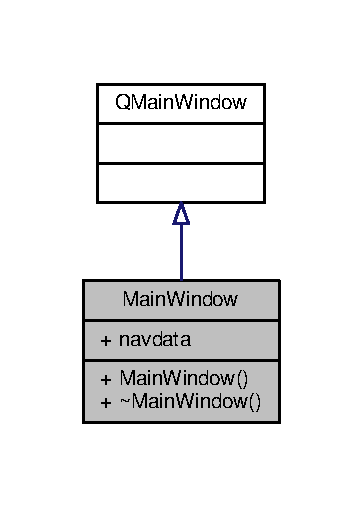
\includegraphics[width=174pt]{class_main_window__inherit__graph}
\end{center}
\end{figure}


Graphe de collaboration de Main\-Window\-:
\nopagebreak
\begin{figure}[H]
\begin{center}
\leavevmode
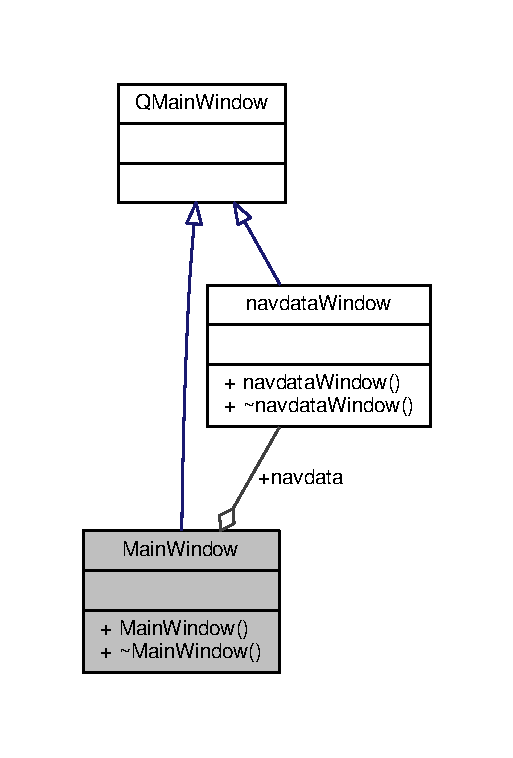
\includegraphics[width=246pt]{class_main_window__coll__graph}
\end{center}
\end{figure}
\subsection*{Fonctions membres publiques}
\begin{DoxyCompactItemize}
\item 
\hyperlink{class_main_window_a46f32c7a0b51359e13505396ce9b316b}{Main\-Window} (Q\-Widget $\ast$parent=0)
\item 
\hyperlink{class_main_window_aa33fa7d45aa34b9ede5cb69ab574a1b2}{$\sim$\-Main\-Window} ()
\end{DoxyCompactItemize}
\subsection*{Champs de données}
\begin{DoxyCompactItemize}
\item 
\hyperlink{classnavdata_window}{navdata\-Window} $\ast$ \hyperlink{class_main_window_a2e8ccc2fc320190b3aed244f54822982}{navdata}
\end{DoxyCompactItemize}


\subsection{Description détaillée}


Définition à la ligne 13 du fichier mainwindow.\-h.



\subsection{Documentation des constructeurs et destructeur}
\hypertarget{class_main_window_a46f32c7a0b51359e13505396ce9b316b}{\index{Main\-Window@{Main\-Window}!Main\-Window@{Main\-Window}}
\index{Main\-Window@{Main\-Window}!MainWindow@{Main\-Window}}
\subsubsection[{Main\-Window}]{\setlength{\rightskip}{0pt plus 5cm}{\bf Main\-Window} (
\begin{DoxyParamCaption}
\item[{Q\-Widget $\ast$}]{parent = {\ttfamily 0}}
\end{DoxyParamCaption}
)\hspace{0.3cm}{\ttfamily [explicit]}}}\label{class_main_window_a46f32c7a0b51359e13505396ce9b316b}


Définition à la ligne 4 du fichier mainwindow.\-cpp.

\hypertarget{class_main_window_aa33fa7d45aa34b9ede5cb69ab574a1b2}{\index{Main\-Window@{Main\-Window}!$\sim$\-Main\-Window@{$\sim$\-Main\-Window}}
\index{$\sim$\-Main\-Window@{$\sim$\-Main\-Window}!MainWindow@{Main\-Window}}
\subsubsection[{$\sim$\-Main\-Window}]{\setlength{\rightskip}{0pt plus 5cm}$\sim${\bf Main\-Window} (
\begin{DoxyParamCaption}
{}
\end{DoxyParamCaption}
)}}\label{class_main_window_aa33fa7d45aa34b9ede5cb69ab574a1b2}


Définition à la ligne 13 du fichier mainwindow.\-cpp.



\subsection{Documentation des champs}
\hypertarget{class_main_window_a2e8ccc2fc320190b3aed244f54822982}{\index{Main\-Window@{Main\-Window}!navdata@{navdata}}
\index{navdata@{navdata}!MainWindow@{Main\-Window}}
\subsubsection[{navdata}]{\setlength{\rightskip}{0pt plus 5cm}{\bf navdata\-Window}$\ast$ navdata}}\label{class_main_window_a2e8ccc2fc320190b3aed244f54822982}


Définition à la ligne 19 du fichier mainwindow.\-h.



La documentation de cette classe a été générée à partir des fichiers suivants \-:\begin{DoxyCompactItemize}
\item 
/media/\-D\-E\-V\-E\-L/\-Projet\-I\-U\-T/\-Drone\-Wifi/sources/keyboard\-Command/\hyperlink{mainwindow_8h}{mainwindow.\-h}\item 
/media/\-D\-E\-V\-E\-L/\-Projet\-I\-U\-T/\-Drone\-Wifi/sources/keyboard\-Command/\hyperlink{mainwindow_8cpp}{mainwindow.\-cpp}\end{DoxyCompactItemize}

\hypertarget{classnavdata_window}{\section{Référence de la classe navdata\-Window}
\label{classnavdata_window}\index{navdata\-Window@{navdata\-Window}}
}


{\ttfamily \#include $<$navdatawindow.\-h$>$}



Graphe d'héritage de navdata\-Window\-:
\nopagebreak
\begin{figure}[H]
\begin{center}
\leavevmode
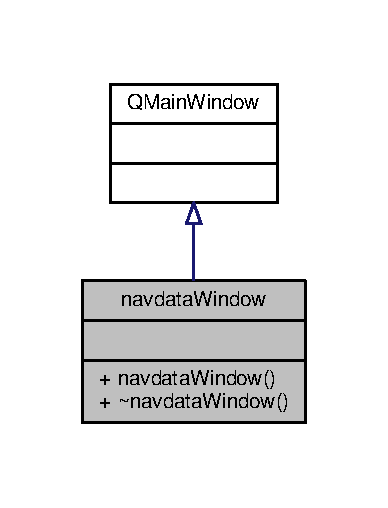
\includegraphics[width=186pt]{classnavdata_window__inherit__graph}
\end{center}
\end{figure}


Graphe de collaboration de navdata\-Window\-:
\nopagebreak
\begin{figure}[H]
\begin{center}
\leavevmode
\includegraphics[width=186pt]{classnavdata_window__coll__graph}
\end{center}
\end{figure}
\subsection*{Fonctions membres publiques}
\begin{DoxyCompactItemize}
\item 
\hyperlink{classnavdata_window_a5e017b35b55ad954e54244cc284b1f5a}{navdata\-Window} (Q\-Widget $\ast$parent=0)
\item 
\hyperlink{classnavdata_window_a33a8fdbabc0661a1ee5c18c7de33440e}{$\sim$navdata\-Window} ()
\end{DoxyCompactItemize}


\subsection{Description détaillée}


Définition à la ligne 11 du fichier navdatawindow.\-h.



\subsection{Documentation des constructeurs et destructeur}
\hypertarget{classnavdata_window_a5e017b35b55ad954e54244cc284b1f5a}{\index{navdata\-Window@{navdata\-Window}!navdata\-Window@{navdata\-Window}}
\index{navdata\-Window@{navdata\-Window}!navdataWindow@{navdata\-Window}}
\subsubsection[{navdata\-Window}]{\setlength{\rightskip}{0pt plus 5cm}{\bf navdata\-Window} (
\begin{DoxyParamCaption}
\item[{Q\-Widget $\ast$}]{parent = {\ttfamily 0}}
\end{DoxyParamCaption}
)\hspace{0.3cm}{\ttfamily [explicit]}}}\label{classnavdata_window_a5e017b35b55ad954e54244cc284b1f5a}


Définition à la ligne 4 du fichier navdatawindow.\-cpp.



Voici le graphe d'appel pour cette fonction \-:
\nopagebreak
\begin{figure}[H]
\begin{center}
\leavevmode
\includegraphics[width=338pt]{classnavdata_window_a5e017b35b55ad954e54244cc284b1f5a_cgraph}
\end{center}
\end{figure}


\hypertarget{classnavdata_window_a33a8fdbabc0661a1ee5c18c7de33440e}{\index{navdata\-Window@{navdata\-Window}!$\sim$navdata\-Window@{$\sim$navdata\-Window}}
\index{$\sim$navdata\-Window@{$\sim$navdata\-Window}!navdataWindow@{navdata\-Window}}
\subsubsection[{$\sim$navdata\-Window}]{\setlength{\rightskip}{0pt plus 5cm}$\sim${\bf navdata\-Window} (
\begin{DoxyParamCaption}
{}
\end{DoxyParamCaption}
)}}\label{classnavdata_window_a33a8fdbabc0661a1ee5c18c7de33440e}


Définition à la ligne 14 du fichier navdatawindow.\-cpp.



La documentation de cette classe a été générée à partir des fichiers suivants \-:\begin{DoxyCompactItemize}
\item 
/media/\-D\-E\-V\-E\-L/\-Projet\-I\-U\-T/\-Drone\-Wifi/sources/keyboard\-Command/\hyperlink{navdatawindow_8h}{navdatawindow.\-h}\item 
/media/\-D\-E\-V\-E\-L/\-Projet\-I\-U\-T/\-Drone\-Wifi/sources/keyboard\-Command/\hyperlink{navdatawindow_8cpp}{navdatawindow.\-cpp}\end{DoxyCompactItemize}

\hypertarget{class_q_main_window}{\section{Référence de la classe Q\-Main\-Window}
\label{class_q_main_window}\index{Q\-Main\-Window@{Q\-Main\-Window}}
}


Graphe d'héritage de Q\-Main\-Window\-:
\nopagebreak
\begin{figure}[H]
\begin{center}
\leavevmode
\includegraphics[width=299pt]{class_q_main_window__inherit__graph}
\end{center}
\end{figure}


Graphe de collaboration de Q\-Main\-Window\-:
\nopagebreak
\begin{figure}[H]
\begin{center}
\leavevmode
\includegraphics[width=160pt]{class_q_main_window__coll__graph}
\end{center}
\end{figure}


La documentation de cette classe a été générée à partir du fichier suivant \-:\begin{DoxyCompactItemize}
\item 
/media/\-D\-E\-V\-E\-L/\-Projet\-I\-U\-T/\-Drone\-Wifi/sources/keyboard\-Command/\hyperlink{mainwindow_8h}{mainwindow.\-h}\end{DoxyCompactItemize}

\hypertarget{class_q_thread}{\section{Référence de la classe Q\-Thread}
\label{class_q_thread}\index{Q\-Thread@{Q\-Thread}}
}


Graphe d'héritage de Q\-Thread\-:
\nopagebreak
\begin{figure}[H]
\begin{center}
\leavevmode
\includegraphics[width=184pt]{class_q_thread__inherit__graph}
\end{center}
\end{figure}


Graphe de collaboration de Q\-Thread\-:
\nopagebreak
\begin{figure}[H]
\begin{center}
\leavevmode
\includegraphics[width=134pt]{class_q_thread__coll__graph}
\end{center}
\end{figure}


La documentation de cette classe a été générée à partir du fichier suivant \-:\begin{DoxyCompactItemize}
\item 
/media/\-D\-E\-V\-E\-L/\-Projet\-I\-U\-T/\-Drone\-Wifi/sources/keyboard\-Command/\hyperlink{ardrone_8h}{ardrone.\-h}\end{DoxyCompactItemize}

\chapter{Documentation des fichiers}
\hypertarget{ardrone_8cpp}{\section{Référence du fichier /media/\-D\-E\-V\-E\-L/\-Projet\-I\-U\-T/\-Drone\-Wifi/sources/keyboard\-Command/ardrone.cpp}
\label{ardrone_8cpp}\index{/media/\-D\-E\-V\-E\-L/\-Projet\-I\-U\-T/\-Drone\-Wifi/sources/keyboard\-Command/ardrone.\-cpp@{/media/\-D\-E\-V\-E\-L/\-Projet\-I\-U\-T/\-Drone\-Wifi/sources/keyboard\-Command/ardrone.\-cpp}}
}
{\ttfamily \#include \char`\"{}ardrone.\-h\char`\"{}}\\*
Graphe des dépendances par inclusion de ardrone.\-cpp\-:
\nopagebreak
\begin{figure}[H]
\begin{center}
\leavevmode
\includegraphics[width=289pt]{ardrone_8cpp__incl}
\end{center}
\end{figure}

\hypertarget{ardrone_8h}{\section{Référence du fichier /media/\-D\-E\-V\-E\-L/\-Projet\-I\-U\-T/\-Drone\-Wifi/sources/keyboard\-Command/ardrone.h}
\label{ardrone_8h}\index{/media/\-D\-E\-V\-E\-L/\-Projet\-I\-U\-T/\-Drone\-Wifi/sources/keyboard\-Command/ardrone.\-h@{/media/\-D\-E\-V\-E\-L/\-Projet\-I\-U\-T/\-Drone\-Wifi/sources/keyboard\-Command/ardrone.\-h}}
}
{\ttfamily \#include $<$Q\-Thread$>$}\\*
{\ttfamily \#include $<$Qt\-Network/\-Q\-Udp\-Socket$>$}\\*
Graphe des dépendances par inclusion de ardrone.\-h\-:
\nopagebreak
\begin{figure}[H]
\begin{center}
\leavevmode
\includegraphics[width=289pt]{ardrone_8h__incl}
\end{center}
\end{figure}
Ce graphe montre quels fichiers incluent directement ou indirectement ce fichier \-:
\nopagebreak
\begin{figure}[H]
\begin{center}
\leavevmode
\includegraphics[width=350pt]{ardrone_8h__dep__incl}
\end{center}
\end{figure}
\subsection*{Structures de données}
\begin{DoxyCompactItemize}
\item 
class \hyperlink{class_a_r_drone}{A\-R\-Drone}
\end{DoxyCompactItemize}

\hypertarget{main_8cpp}{\section{Référence du fichier /media/\-D\-E\-V\-E\-L/\-Projet\-I\-U\-T/\-Drone\-Wifi/sources/keyboard\-Command/main.cpp}
\label{main_8cpp}\index{/media/\-D\-E\-V\-E\-L/\-Projet\-I\-U\-T/\-Drone\-Wifi/sources/keyboard\-Command/main.\-cpp@{/media/\-D\-E\-V\-E\-L/\-Projet\-I\-U\-T/\-Drone\-Wifi/sources/keyboard\-Command/main.\-cpp}}
}
{\ttfamily \#include \char`\"{}mainwindow.\-h\char`\"{}}\\*
{\ttfamily \#include $<$Q\-Application$>$}\\*
Graphe des dépendances par inclusion de main.\-cpp\-:
\nopagebreak
\begin{figure}[H]
\begin{center}
\leavevmode
\includegraphics[width=350pt]{main_8cpp__incl}
\end{center}
\end{figure}
\subsection*{Fonctions}
\begin{DoxyCompactItemize}
\item 
int \hyperlink{main_8cpp_a0ddf1224851353fc92bfbff6f499fa97}{main} (int argc, char $\ast$argv\mbox{[}$\,$\mbox{]})
\end{DoxyCompactItemize}


\subsection{Documentation des fonctions}
\hypertarget{main_8cpp_a0ddf1224851353fc92bfbff6f499fa97}{\index{main.\-cpp@{main.\-cpp}!main@{main}}
\index{main@{main}!main.cpp@{main.\-cpp}}
\subsubsection[{main}]{\setlength{\rightskip}{0pt plus 5cm}int main (
\begin{DoxyParamCaption}
\item[{int}]{argc, }
\item[{char $\ast$}]{argv\mbox{[}$\,$\mbox{]}}
\end{DoxyParamCaption}
)}}\label{main_8cpp_a0ddf1224851353fc92bfbff6f499fa97}


Définition à la ligne 4 du fichier main.\-cpp.


\hypertarget{mainwindow_8cpp}{\section{Référence du fichier /media/\-D\-E\-V\-E\-L/\-Projet\-I\-U\-T/\-Drone\-Wifi/sources/keyboard\-Command/mainwindow.cpp}
\label{mainwindow_8cpp}\index{/media/\-D\-E\-V\-E\-L/\-Projet\-I\-U\-T/\-Drone\-Wifi/sources/keyboard\-Command/mainwindow.\-cpp@{/media/\-D\-E\-V\-E\-L/\-Projet\-I\-U\-T/\-Drone\-Wifi/sources/keyboard\-Command/mainwindow.\-cpp}}
}
{\ttfamily \#include \char`\"{}mainwindow.\-h\char`\"{}}\\*
{\ttfamily \#include \char`\"{}ui\-\_\-mainwindow.\-h\char`\"{}}\\*
Graphe des dépendances par inclusion de mainwindow.\-cpp\-:
\nopagebreak
\begin{figure}[H]
\begin{center}
\leavevmode
\includegraphics[width=350pt]{mainwindow_8cpp__incl}
\end{center}
\end{figure}

\hypertarget{mainwindow_8h}{\section{Référence du fichier /media/\-D\-E\-V\-E\-L/\-Projet\-I\-U\-T/\-Drone\-Wifi/sources/keyboard\-Command/mainwindow.h}
\label{mainwindow_8h}\index{/media/\-D\-E\-V\-E\-L/\-Projet\-I\-U\-T/\-Drone\-Wifi/sources/keyboard\-Command/mainwindow.\-h@{/media/\-D\-E\-V\-E\-L/\-Projet\-I\-U\-T/\-Drone\-Wifi/sources/keyboard\-Command/mainwindow.\-h}}
}
{\ttfamily \#include $<$Q\-Main\-Window$>$}\\*
{\ttfamily \#include $<$Q\-Key\-Event$>$}\\*
{\ttfamily \#include \char`\"{}ardrone.\-h\char`\"{}}\\*
{\ttfamily \#include \char`\"{}navdatawindow.\-h\char`\"{}}\\*
Graphe des dépendances par inclusion de mainwindow.\-h\-:
\nopagebreak
\begin{figure}[H]
\begin{center}
\leavevmode
\includegraphics[width=350pt]{mainwindow_8h__incl}
\end{center}
\end{figure}
Ce graphe montre quels fichiers incluent directement ou indirectement ce fichier \-:
\nopagebreak
\begin{figure}[H]
\begin{center}
\leavevmode
\includegraphics[width=350pt]{mainwindow_8h__dep__incl}
\end{center}
\end{figure}
\subsection*{Classes}
\begin{DoxyCompactItemize}
\item 
class \hyperlink{class_main_window}{Main\-Window}
\end{DoxyCompactItemize}
\subsection*{Espaces de nommage}
\begin{DoxyCompactItemize}
\item 
namespace \hyperlink{namespace_ui}{Ui}
\end{DoxyCompactItemize}

\hypertarget{navdatawindow_8cpp}{\section{Référence du fichier /media/\-D\-E\-V\-E\-L/\-Projet\-I\-U\-T/\-Drone\-Wifi/sources/keyboard\-Command/navdatawindow.cpp}
\label{navdatawindow_8cpp}\index{/media/\-D\-E\-V\-E\-L/\-Projet\-I\-U\-T/\-Drone\-Wifi/sources/keyboard\-Command/navdatawindow.\-cpp@{/media/\-D\-E\-V\-E\-L/\-Projet\-I\-U\-T/\-Drone\-Wifi/sources/keyboard\-Command/navdatawindow.\-cpp}}
}
{\ttfamily \#include \char`\"{}navdatawindow.\-h\char`\"{}}\\*
{\ttfamily \#include \char`\"{}ui\-\_\-navdatawindow.\-h\char`\"{}}\\*
Graphe des dépendances par inclusion de navdatawindow.\-cpp\-:
\nopagebreak
\begin{figure}[H]
\begin{center}
\leavevmode
\includegraphics[width=332pt]{navdatawindow_8cpp__incl}
\end{center}
\end{figure}

\hypertarget{navdatawindow_8h}{\section{Référence du fichier /media/\-D\-E\-V\-E\-L/\-Projet\-I\-U\-T/\-Drone\-Wifi/sources/keyboard\-Command/navdatawindow.h}
\label{navdatawindow_8h}\index{/media/\-D\-E\-V\-E\-L/\-Projet\-I\-U\-T/\-Drone\-Wifi/sources/keyboard\-Command/navdatawindow.\-h@{/media/\-D\-E\-V\-E\-L/\-Projet\-I\-U\-T/\-Drone\-Wifi/sources/keyboard\-Command/navdatawindow.\-h}}
}
{\ttfamily \#include $<$Q\-Main\-Window$>$}\\*
{\ttfamily \#include \char`\"{}ardrone.\-h\char`\"{}}\\*
Graphe des dépendances par inclusion de navdatawindow.\-h\-:
\nopagebreak
\begin{figure}[H]
\begin{center}
\leavevmode
\includegraphics[width=333pt]{navdatawindow_8h__incl}
\end{center}
\end{figure}
Ce graphe montre quels fichiers incluent directement ou indirectement ce fichier \-:
\nopagebreak
\begin{figure}[H]
\begin{center}
\leavevmode
\includegraphics[width=350pt]{navdatawindow_8h__dep__incl}
\end{center}
\end{figure}
\subsection*{Classes}
\begin{DoxyCompactItemize}
\item 
class \hyperlink{classnavdata_window}{navdata\-Window}
\end{DoxyCompactItemize}
\subsection*{Espaces de nommage}
\begin{DoxyCompactItemize}
\item 
namespace \hyperlink{namespace_ui}{Ui}
\end{DoxyCompactItemize}

\hypertarget{connexion_8c}{\section{Référence du fichier /media/\-D\-E\-V\-E\-L/\-Projet\-I\-U\-T/\-Drone\-Wifi/sources/wifi/connexion.c}
\label{connexion_8c}\index{/media/\-D\-E\-V\-E\-L/\-Projet\-I\-U\-T/\-Drone\-Wifi/sources/wifi/connexion.\-c@{/media/\-D\-E\-V\-E\-L/\-Projet\-I\-U\-T/\-Drone\-Wifi/sources/wifi/connexion.\-c}}
}
\subsection*{Structures de données}
\begin{DoxyCompactItemize}
\item 
struct \hyperlink{structetat__commandes}{etat\-\_\-commandes}
\item 
struct \hyperlink{structardrone}{ardrone}
\end{DoxyCompactItemize}
\subsection*{Macros}
\begin{DoxyCompactItemize}
\item 
\#define \hyperlink{connexion_8c_af46219462f0da78b25d5d693e325f865}{L\-O\-C\-A\-L\-\_\-\-P\-O\-R\-T}~5556
\item 
\#define \hyperlink{connexion_8c_ab1adf860adf915687d9063e8a19fc2a6}{R\-E\-M\-O\-T\-E\-\_\-\-I\-P}~\char`\"{}255.\-255.\-255.\-255\char`\"{} /$\ast$broadcast$\ast$/
\item 
\#define \hyperlink{connexion_8c_aa27dfcf9c5badbcdb4f87febf8ffed8d}{R\-E\-M\-O\-T\-E\-\_\-\-P\-O\-R\-T}~\hyperlink{connexion_8c_af46219462f0da78b25d5d693e325f865}{L\-O\-C\-A\-L\-\_\-\-P\-O\-R\-T}
\item 
\#define \hyperlink{connexion_8c_a13322faf91898e76cf7857e23136615d}{T\-C\-P\-C\-O\-N\-F\-I\-G}~5
\item 
\#define \hyperlink{connexion_8c_a972172a830ac4cb6319037de9fdcec96}{I\-P\-D\-R\-O\-N\-E}~\char`\"{}192.\-168.\-1.\-1\char`\"{}
\item 
\#define \hyperlink{connexion_8c_a41f9c5fb8b08eb5dc3edce4dcb37fee7}{true}~(1)
\item 
\#define \hyperlink{connexion_8c_a65e9886d74aaee76545e83dd09011727}{false}~(0)
\item 
\#define \hyperlink{group___a_t_commands_ga58b930fb43c5cd2fc89a84647e6fe51c}{cppbool}~char
\begin{DoxyCompactList}\small\item\em Implementation du type c++ bool en c. \end{DoxyCompactList}\item 
\#define \hyperlink{group___i_o_gad8d73a31b3d7e5ed74e525e198cc78f3}{c\-W\-A\-I\-T\-\_\-5\-\_\-us}
\begin{DoxyCompactList}\small\item\em pause de 5 µs \end{DoxyCompactList}\end{DoxyCompactItemize}
\subsection*{Énumérations}
\begin{DoxyCompactItemize}
\item 
enum \hyperlink{connexion_8c_a6e7539fec119487042de45d22b1efca7}{statut\-\_\-connexion} \{ \hyperlink{connexion_8c_a6e7539fec119487042de45d22b1efca7a66a4cbb7d89a1ddbd9a1df3a0484ac24}{I\-N\-O\-C\-C\-U\-P\-E}, 
\hyperlink{connexion_8c_a6e7539fec119487042de45d22b1efca7ae33abe2273c178ffb3f8567308ee831d}{R\-E\-C\-H\-E\-R\-C\-H\-E}, 
\hyperlink{connexion_8c_a6e7539fec119487042de45d22b1efca7a50404969b4b67c138ceb4d93314d9fea}{T\-R\-O\-U\-V\-E}, 
\hyperlink{connexion_8c_a6e7539fec119487042de45d22b1efca7a0c8506530b77c355a33f900ed83b8e06}{C\-O\-N\-N\-E\-C\-T\-E}
 \}
\end{DoxyCompactItemize}
\subsection*{Fonctions}
\begin{DoxyCompactItemize}
\item 
void \hyperlink{group___i_o_ga9cb15ec1781380780672afe306a163ec}{B\-R\-D\-Init} (void)
\begin{DoxyCompactList}\small\item\em Initialise tous les ports d'entreés sorties pour la carte joystick. \end{DoxyCompactList}\item 
void \hyperlink{group___i_o_gaba1669c59c764f752e4759af60633240}{print\-\_\-etat\-\_\-commandes} (\hyperlink{structetat__commandes}{etat\-\_\-commandes} s)
\begin{DoxyCompactList}\small\item\em initialise la structure structure de l'état des commandes \end{DoxyCompactList}\item 
void \hyperlink{group___i_o_ga47503442984c9244a27e7b95ffa472c3}{init\-\_\-etat\-\_\-commandes} (\hyperlink{structetat__commandes}{etat\-\_\-commandes} $\ast$s)
\begin{DoxyCompactList}\small\item\em initialise la structure structure de l'état des commandes \end{DoxyCompactList}\item 
void \hyperlink{group___i_o_gaf61e8f99c1568bc62cd24251e4cc0fa2}{S\-P\-I\-\_\-\-C\-L\-K} (char v)
\begin{DoxyCompactList}\small\item\em modifie l'état de la sortie C\-L\-K pour le convertisseur A/\-N S\-P\-I \end{DoxyCompactList}\item 
void \hyperlink{group___i_o_ga831fe77ab7ce75ba9a41ecb3c08a97d9}{S\-P\-I\-\_\-\-D\-I\-N} (char v)
\begin{DoxyCompactList}\small\item\em modifie l'état de la sortie D\-I\-N pour le convertisseur A/\-N S\-P\-I \end{DoxyCompactList}\item 
void \hyperlink{group___i_o_gab5cfdcd0547c9f87516a805b4849d64f}{S\-P\-I\-\_\-\-C\-S} (char v)
\begin{DoxyCompactList}\small\item\em modifie l'état de la sortie C\-S pour le convertisseur A/\-N S\-P\-I \end{DoxyCompactList}\item 
int \hyperlink{group___i_o_ga837457e63fcbfcc6e59b6d4c59bd7252}{S\-P\-I\-\_\-\-D\-O\-U\-T} (void)
\begin{DoxyCompactList}\small\item\em lit l'état de l'entrée D\-O\-U\-T du convertisseur A/\-N S\-P\-I \end{DoxyCompactList}\item 
void \hyperlink{group___i_o_ga2574e1f1506d0a5313c21891bef79aca}{S\-P\-I\-\_\-delay} (int i)
\begin{DoxyCompactList}\small\item\em temps d'attente de 'i' $\ast$ 5 µs \end{DoxyCompactList}\item 
int \hyperlink{group___i_o_ga5232f075d5cd2577d072721a1494eb03}{S\-P\-Iread} (char addr)
\begin{DoxyCompactList}\small\item\em demande au convertisseur A/\-N S\-P\-I de convertir le canal addr \end{DoxyCompactList}\item 
void \hyperlink{group___i_o_ga91ea6d792c13305827a81e66a1eedf87}{lire\-Commandes} (\hyperlink{structetat__commandes}{etat\-\_\-commandes} $\ast$s)
\begin{DoxyCompactList}\small\item\em remplie la structure de l'état des commandes avec de nouvelles valeurs lues \end{DoxyCompactList}\item 
void \hyperlink{group___i_o_ga85dc4c920777870405563fe56611b457}{ecrire\-Commandes} (\hyperlink{structetat__commandes}{etat\-\_\-commandes} s)
\begin{DoxyCompactList}\small\item\em écris les valeurs de la structure de l'état des commandes en sortie. \end{DoxyCompactList}\item 
\hyperlink{group___a_t_commands_ga58b930fb43c5cd2fc89a84647e6fe51c}{cppbool} \hyperlink{group___u_d_p_ga303d5a717d50385e7908c735d5bddff7}{send\-\_\-packet} (char $\ast$str, const char far $\ast$ip, word port, udp\-\_\-\-Socket $\ast$sock)
\begin{DoxyCompactList}\small\item\em envoie une chaîne de caractère \end{DoxyCompactList}\item 
int \hyperlink{group___connexion_ga933f44b3a816d407be7ad49f7544342e}{rxsignal\-\_\-cmp} (far \-\_\-wifi\-\_\-wln\-\_\-scan\-\_\-bss $\ast$a, far \-\_\-wifi\-\_\-wln\-\_\-scan\-\_\-bss $\ast$b)
\begin{DoxyCompactList}\small\item\em fonction qui permet le trie les points d'accès Wi\-Fi par puissance du signal \end{DoxyCompactList}\item 
root void \hyperlink{group___connexion_gad60eefc83c0bcc85273af32869e49f5d}{scan\-\_\-assoc\-\_\-callback} (far wifi\-\_\-scan\-\_\-data $\ast$data)
\begin{DoxyCompactList}\small\item\em fonction de callback qui traite les points d'accès donnés \-: recherche le point d'accès du drone et se connecte \end{DoxyCompactList}\item 
void \hyperlink{group___connexion_ga4316deed036a20c32186612b0e2ed7f2}{connexion} (void)
\begin{DoxyCompactList}\small\item\em fonction qui se connecte au drone. Elle se quitte uniquement si la connexion est effective \end{DoxyCompactList}\item 
\hyperlink{group___a_t_commands_ga58b930fb43c5cd2fc89a84647e6fe51c}{cppbool} \hyperlink{group___a_t_commands_gab107cb405a02a0e16ee50f68347c6d4d}{connect\-To\-Drone} (far \hyperlink{structardrone}{ardrone} $\ast$dr)
\begin{DoxyCompactList}\small\item\em Initie la connexion avec le drone dr. \end{DoxyCompactList}\item 
\hyperlink{group___a_t_commands_ga58b930fb43c5cd2fc89a84647e6fe51c}{cppbool} \hyperlink{group___a_t_commands_ga4daa3ada04813c5a99503bd329c6be2c}{init\-Drone} (far \hyperlink{structardrone}{ardrone} $\ast$dr)
\begin{DoxyCompactList}\small\item\em Initialisation du drone dr pour permettre un décollage en toute sécurité. \end{DoxyCompactList}\item 
\hyperlink{group___a_t_commands_ga58b930fb43c5cd2fc89a84647e6fe51c}{cppbool} \hyperlink{group___a_t_commands_ga565736370f76ee54efe74f65acb3ccc4}{takeoff} (far \hyperlink{structardrone}{ardrone} $\ast$dr)
\begin{DoxyCompactList}\small\item\em Commande le décollage du drone dr. \end{DoxyCompactList}\item 
\hyperlink{group___a_t_commands_ga58b930fb43c5cd2fc89a84647e6fe51c}{cppbool} \hyperlink{group___a_t_commands_ga89c4cd20c1bb10d5624cdcc2154efdd1}{land} (far \hyperlink{structardrone}{ardrone} $\ast$dr)
\begin{DoxyCompactList}\small\item\em Commande l'atterissage du drone dr. \end{DoxyCompactList}\item 
\hyperlink{group___a_t_commands_ga58b930fb43c5cd2fc89a84647e6fe51c}{cppbool} \hyperlink{group___a_t_commands_gab16c7bf6e0f5d8df9f422308cb958b2d}{aru} (far \hyperlink{structardrone}{ardrone} $\ast$dr)
\begin{DoxyCompactList}\small\item\em Envoi un arrêt d'urgence au drone dr. \end{DoxyCompactList}\item 
\hyperlink{group___a_t_commands_ga58b930fb43c5cd2fc89a84647e6fe51c}{cppbool} \hyperlink{group___a_t_commands_gafba5305bd996ecb4332a17cf68e79928}{vol\-Command} (far \hyperlink{structardrone}{ardrone} $\ast$dr, float tilt\-Left\-Right\-\_\-, float tilt\-Front\-Back\-\_\-, float go\-Up\-Down\-\_\-, float turn\-Left\-Right\-\_\-)
\begin{DoxyCompactList}\small\item\em Envoi de la commande de vol au drone dr. \end{DoxyCompactList}\item 
void \hyperlink{group___a_t_commands_ga9d9aece95d737ed64ba8e9131ff0065c}{set\-Go\-Up\-Down} (far \hyperlink{structardrone}{ardrone} $\ast$dr, float val)
\begin{DoxyCompactList}\small\item\em Mettre une valeur de manière sécurisée dans le buffer de la vitesse verticale du drone dr. \end{DoxyCompactList}\item 
void \hyperlink{group___a_t_commands_ga0d757863caf7f9c4110ab6e71cac1a4c}{set\-Turn\-Left\-Right} (far \hyperlink{structardrone}{ardrone} $\ast$dr, float val)
\begin{DoxyCompactList}\small\item\em Mettre une valeur dans de manière sécurisée dans le buffer de la vitesse angulaire du drone dr. \end{DoxyCompactList}\item 
void \hyperlink{group___a_t_commands_ga9a290eee046f983fc53d282c0bc53aff}{set\-Tilt\-Front\-Back} (far \hyperlink{structardrone}{ardrone} $\ast$dr, float val)
\begin{DoxyCompactList}\small\item\em Mettre une valeur de manière sécurisé dans le buffer de l'inclinaison avant/arrière du drone dr. \end{DoxyCompactList}\item 
void \hyperlink{group___a_t_commands_ga28a6f7458f7dbcdf7068b26236f10e2c}{set\-Tilt\-Left\-Right} (far \hyperlink{structardrone}{ardrone} $\ast$dr, float val)
\begin{DoxyCompactList}\small\item\em Mettre une valeur de manière sécurisée dans le buffer de l'inclinaison gauche/droite du drone dr. \end{DoxyCompactList}\item 
\hyperlink{group___a_t_commands_ga58b930fb43c5cd2fc89a84647e6fe51c}{cppbool} \hyperlink{group___a_t_commands_gad4a88a78f2b094bcce69b749a845e11c}{send\-A\-T} (far \hyperlink{structardrone}{ardrone} $\ast$dr)
\begin{DoxyCompactList}\small\item\em Envoyer la commande A\-T qui est dans le buffer du drone dr. \end{DoxyCompactList}\item 
far \hyperlink{structardrone}{ardrone} $\ast$ \hyperlink{group___a_t_commands_ga6f1e46bbcb882594c8442c75ae3dedf8}{new\-A\-R\-Drone} (void)
\begin{DoxyCompactList}\small\item\em Constructeur de l'objet ardrone. \end{DoxyCompactList}\item 
void \hyperlink{group___a_t_commands_gad550dbbb88a791f7e8d64c801ce06bf6}{close\-A\-R\-Drone} (far \hyperlink{structardrone}{ardrone} $\ast$dr)
\begin{DoxyCompactList}\small\item\em Destructeur de l'objet ardrone. \end{DoxyCompactList}\item 
void \hyperlink{connexion_8c_a6288eba0f8e8ad3ab1544ad731eb7667}{main} (void)
\begin{DoxyCompactList}\small\item\em Fonction principal \-: gestion du pilotage du drone en fonctions des entrées/sorties. \end{DoxyCompactList}\end{DoxyCompactItemize}
\subsection*{Variables}
\begin{DoxyCompactItemize}
\item 
\hyperlink{connexion_8c_a6e7539fec119487042de45d22b1efca7}{statut\-\_\-connexion} \hyperlink{connexion_8c_a6c0592b34aa72ee716e9c0b939038faa}{connect} = \hyperlink{connexion_8c_a6e7539fec119487042de45d22b1efca7a66a4cbb7d89a1ddbd9a1df3a0484ac24}{I\-N\-O\-C\-C\-U\-P\-E}
\end{DoxyCompactItemize}


\subsection{Documentation des macros}
\hypertarget{connexion_8c_a65e9886d74aaee76545e83dd09011727}{\index{connexion.\-c@{connexion.\-c}!false@{false}}
\index{false@{false}!connexion.c@{connexion.\-c}}
\subsubsection[{false}]{\setlength{\rightskip}{0pt plus 5cm}\#define false~(0)}}\label{connexion_8c_a65e9886d74aaee76545e83dd09011727}


Définition à la ligne 82 du fichier connexion.\-c.

\hypertarget{connexion_8c_a972172a830ac4cb6319037de9fdcec96}{\index{connexion.\-c@{connexion.\-c}!I\-P\-D\-R\-O\-N\-E@{I\-P\-D\-R\-O\-N\-E}}
\index{I\-P\-D\-R\-O\-N\-E@{I\-P\-D\-R\-O\-N\-E}!connexion.c@{connexion.\-c}}
\subsubsection[{I\-P\-D\-R\-O\-N\-E}]{\setlength{\rightskip}{0pt plus 5cm}\#define I\-P\-D\-R\-O\-N\-E~\char`\"{}192.\-168.\-1.\-1\char`\"{}}}\label{connexion_8c_a972172a830ac4cb6319037de9fdcec96}


Définition à la ligne 37 du fichier connexion.\-c.

\hypertarget{connexion_8c_af46219462f0da78b25d5d693e325f865}{\index{connexion.\-c@{connexion.\-c}!L\-O\-C\-A\-L\-\_\-\-P\-O\-R\-T@{L\-O\-C\-A\-L\-\_\-\-P\-O\-R\-T}}
\index{L\-O\-C\-A\-L\-\_\-\-P\-O\-R\-T@{L\-O\-C\-A\-L\-\_\-\-P\-O\-R\-T}!connexion.c@{connexion.\-c}}
\subsubsection[{L\-O\-C\-A\-L\-\_\-\-P\-O\-R\-T}]{\setlength{\rightskip}{0pt plus 5cm}\#define L\-O\-C\-A\-L\-\_\-\-P\-O\-R\-T~5556}}\label{connexion_8c_af46219462f0da78b25d5d693e325f865}


Définition à la ligne 10 du fichier connexion.\-c.

\hypertarget{connexion_8c_ab1adf860adf915687d9063e8a19fc2a6}{\index{connexion.\-c@{connexion.\-c}!R\-E\-M\-O\-T\-E\-\_\-\-I\-P@{R\-E\-M\-O\-T\-E\-\_\-\-I\-P}}
\index{R\-E\-M\-O\-T\-E\-\_\-\-I\-P@{R\-E\-M\-O\-T\-E\-\_\-\-I\-P}!connexion.c@{connexion.\-c}}
\subsubsection[{R\-E\-M\-O\-T\-E\-\_\-\-I\-P}]{\setlength{\rightskip}{0pt plus 5cm}\#define R\-E\-M\-O\-T\-E\-\_\-\-I\-P~\char`\"{}255.\-255.\-255.\-255\char`\"{} /$\ast$broadcast$\ast$/}}\label{connexion_8c_ab1adf860adf915687d9063e8a19fc2a6}


Définition à la ligne 17 du fichier connexion.\-c.

\hypertarget{connexion_8c_aa27dfcf9c5badbcdb4f87febf8ffed8d}{\index{connexion.\-c@{connexion.\-c}!R\-E\-M\-O\-T\-E\-\_\-\-P\-O\-R\-T@{R\-E\-M\-O\-T\-E\-\_\-\-P\-O\-R\-T}}
\index{R\-E\-M\-O\-T\-E\-\_\-\-P\-O\-R\-T@{R\-E\-M\-O\-T\-E\-\_\-\-P\-O\-R\-T}!connexion.c@{connexion.\-c}}
\subsubsection[{R\-E\-M\-O\-T\-E\-\_\-\-P\-O\-R\-T}]{\setlength{\rightskip}{0pt plus 5cm}\#define R\-E\-M\-O\-T\-E\-\_\-\-P\-O\-R\-T~{\bf L\-O\-C\-A\-L\-\_\-\-P\-O\-R\-T}}}\label{connexion_8c_aa27dfcf9c5badbcdb4f87febf8ffed8d}


Définition à la ligne 20 du fichier connexion.\-c.

\hypertarget{connexion_8c_a13322faf91898e76cf7857e23136615d}{\index{connexion.\-c@{connexion.\-c}!T\-C\-P\-C\-O\-N\-F\-I\-G@{T\-C\-P\-C\-O\-N\-F\-I\-G}}
\index{T\-C\-P\-C\-O\-N\-F\-I\-G@{T\-C\-P\-C\-O\-N\-F\-I\-G}!connexion.c@{connexion.\-c}}
\subsubsection[{T\-C\-P\-C\-O\-N\-F\-I\-G}]{\setlength{\rightskip}{0pt plus 5cm}\#define T\-C\-P\-C\-O\-N\-F\-I\-G~5}}\label{connexion_8c_a13322faf91898e76cf7857e23136615d}


Définition à la ligne 29 du fichier connexion.\-c.

\hypertarget{connexion_8c_a41f9c5fb8b08eb5dc3edce4dcb37fee7}{\index{connexion.\-c@{connexion.\-c}!true@{true}}
\index{true@{true}!connexion.c@{connexion.\-c}}
\subsubsection[{true}]{\setlength{\rightskip}{0pt plus 5cm}\#define true~(1)}}\label{connexion_8c_a41f9c5fb8b08eb5dc3edce4dcb37fee7}


Définition à la ligne 81 du fichier connexion.\-c.



\subsection{Documentation du type de l'énumération}
\hypertarget{connexion_8c_a6e7539fec119487042de45d22b1efca7}{\index{connexion.\-c@{connexion.\-c}!statut\-\_\-connexion@{statut\-\_\-connexion}}
\index{statut\-\_\-connexion@{statut\-\_\-connexion}!connexion.c@{connexion.\-c}}
\subsubsection[{statut\-\_\-connexion}]{\setlength{\rightskip}{0pt plus 5cm}enum {\bf statut\-\_\-connexion}}}\label{connexion_8c_a6e7539fec119487042de45d22b1efca7}
\begin{Desc}
\item[Valeurs énumérées]\par
\begin{description}
\index{I\-N\-O\-C\-C\-U\-P\-E@{I\-N\-O\-C\-C\-U\-P\-E}!connexion.\-c@{connexion.\-c}}\index{connexion.\-c@{connexion.\-c}!I\-N\-O\-C\-C\-U\-P\-E@{I\-N\-O\-C\-C\-U\-P\-E}}\item[{\em 
\hypertarget{connexion_8c_a6e7539fec119487042de45d22b1efca7a66a4cbb7d89a1ddbd9a1df3a0484ac24}{I\-N\-O\-C\-C\-U\-P\-E}\label{connexion_8c_a6e7539fec119487042de45d22b1efca7a66a4cbb7d89a1ddbd9a1df3a0484ac24}
}]\index{R\-E\-C\-H\-E\-R\-C\-H\-E@{R\-E\-C\-H\-E\-R\-C\-H\-E}!connexion.\-c@{connexion.\-c}}\index{connexion.\-c@{connexion.\-c}!R\-E\-C\-H\-E\-R\-C\-H\-E@{R\-E\-C\-H\-E\-R\-C\-H\-E}}\item[{\em 
\hypertarget{connexion_8c_a6e7539fec119487042de45d22b1efca7ae33abe2273c178ffb3f8567308ee831d}{R\-E\-C\-H\-E\-R\-C\-H\-E}\label{connexion_8c_a6e7539fec119487042de45d22b1efca7ae33abe2273c178ffb3f8567308ee831d}
}]\index{T\-R\-O\-U\-V\-E@{T\-R\-O\-U\-V\-E}!connexion.\-c@{connexion.\-c}}\index{connexion.\-c@{connexion.\-c}!T\-R\-O\-U\-V\-E@{T\-R\-O\-U\-V\-E}}\item[{\em 
\hypertarget{connexion_8c_a6e7539fec119487042de45d22b1efca7a50404969b4b67c138ceb4d93314d9fea}{T\-R\-O\-U\-V\-E}\label{connexion_8c_a6e7539fec119487042de45d22b1efca7a50404969b4b67c138ceb4d93314d9fea}
}]\index{C\-O\-N\-N\-E\-C\-T\-E@{C\-O\-N\-N\-E\-C\-T\-E}!connexion.\-c@{connexion.\-c}}\index{connexion.\-c@{connexion.\-c}!C\-O\-N\-N\-E\-C\-T\-E@{C\-O\-N\-N\-E\-C\-T\-E}}\item[{\em 
\hypertarget{connexion_8c_a6e7539fec119487042de45d22b1efca7a0c8506530b77c355a33f900ed83b8e06}{C\-O\-N\-N\-E\-C\-T\-E}\label{connexion_8c_a6e7539fec119487042de45d22b1efca7a0c8506530b77c355a33f900ed83b8e06}
}]\end{description}
\end{Desc}


Définition à la ligne 46 du fichier connexion.\-c.



\subsection{Documentation des fonctions}
\hypertarget{connexion_8c_a6288eba0f8e8ad3ab1544ad731eb7667}{\index{connexion.\-c@{connexion.\-c}!main@{main}}
\index{main@{main}!connexion.c@{connexion.\-c}}
\subsubsection[{main}]{\setlength{\rightskip}{0pt plus 5cm}void main (
\begin{DoxyParamCaption}
\item[{void}]{}
\end{DoxyParamCaption}
)}}\label{connexion_8c_a6288eba0f8e8ad3ab1544ad731eb7667}


Fonction principal \-: gestion du pilotage du drone en fonctions des entrées/sorties. 

\begin{DoxyAuthor}{Auteur}
Baudouin Feildel 
\end{DoxyAuthor}


Définition à la ligne 375 du fichier connexion.\-c.



Voici le graphe d'appel pour cette fonction \-:\nopagebreak
\begin{figure}[H]
\begin{center}
\leavevmode
\includegraphics[width=350pt]{connexion_8c_a6288eba0f8e8ad3ab1544ad731eb7667_cgraph}
\end{center}
\end{figure}




\subsection{Documentation des variables}
\hypertarget{connexion_8c_a6c0592b34aa72ee716e9c0b939038faa}{\index{connexion.\-c@{connexion.\-c}!connect@{connect}}
\index{connect@{connect}!connexion.c@{connexion.\-c}}
\subsubsection[{connect}]{\setlength{\rightskip}{0pt plus 5cm}{\bf statut\-\_\-connexion} connect = {\bf I\-N\-O\-C\-C\-U\-P\-E}}}\label{connexion_8c_a6c0592b34aa72ee716e9c0b939038faa}


Définition à la ligne 89 du fichier connexion.\-c.


\addcontentsline{toc}{part}{Index}
\printindex
\end{document}
